\chapter{Other Debugging Information}
\label{chap:otherdebugginginformation}
% references to chapter 7 look like  {datarep:...}
This section describes debugging information that is not
represented in the form of debugging information entries and
is not contained within a \dotdebuginfo{} section.

In the descriptions that follow, these terms are used to
specify the representation of DWARF sections:
\begin{itemize}

\item
\HFTinitiallength{}, \HFTsectionoffset{} and
\HFTsectionlength{}, which are
defined in
Sections \refersec{datarep:initiallengthvalues} and
\refersec{datarep:32bitand64bitdwarfformats}.

\item
\HFTsbyte{},
\HFTubyte{},
\HFTuhalf{} and
\HFTuword{},
which are defined in
Section \refersec{datarep:integerrepresentationnames}.

\item
\bb
MBZ, which indicates that a value or the contents of a field must be zero.
\eb

\end{itemize}

\section{Accelerated Access}
\label{chap:acceleratedaccess}

\textit{A debugger frequently needs to find the debugging information
\addtoindexx{accelerated access}
for a program entity defined outside of the compilation unit
where the debugged program is currently stopped. Sometimes the
debugger will know only the name of the entity; sometimes only
the address. To find the debugging information associated with
a global entity by name, using the DWARF debugging information
entries alone, a debugger would need to run through all
entries at the highest scope within each compilation unit.}

\textit{Similarly, in languages in which the name of a type is
required to always refer to the same concrete type (such as
C++), a compiler may choose to elide type definitions in
all compilation units except one. In this case a debugger
needs a rapid way of locating the concrete type definition
by name. As with the definition of global data objects, this
would require a search of all the top level type definitions
of all compilation units in a program.}

\needlines{4}
\textit{To find the debugging information associated with a subroutine,
given an address, a debugger can use the low and high PC
attributes of the compilation unit entries to quickly narrow
down the search, but these attributes only cover the range
of addresses for the text associated with a compilation unit
entry. To find the debugging information associated with a
data object, given an address, an exhaustive search would be
needed. Furthermore, any search through debugging information
entries for different compilation units within a large program
would potentially require the access of many memory pages,
probably hurting debugger performance.}

To make lookups of program entities (including data objects,
functions and types) by name or by address faster, a producer
of DWARF information may provide two different types of tables
containing information about the debugging information
entries owned by a particular compilation unit entry in a
more condensed format.

\subsection{Lookup by Name}
\addtoindexx{lookup!by name}
\addtoindexx{accelerated access!by name}
\addtoindexx{name index}
For lookup by name, a name index is maintained in a separate
object file section named \dotdebugnames{}.

\textit{The \dotdebugnames{} section is new in \DWARFVersionV,
and supersedes the \dotdebugpubnames{} and \dotdebugpubtypes{}
sections of earlier DWARF versions. While \dotdebugnames{} and
either \dotdebugpubnames{} and/or \dotdebugpubtypes{} sections
cannot both occur in the same compilation unit, both may be
found in the set of units that make up an executable or shared
object.}

The index consists
primarily of two parts: a list of names, and a list of index
entries. A name, such as a subprogram name, type name, or
variable name, may have several defining declarations in the
debugging information. In this case, the entry for that name in
the list of names will refer to a sequence of index entries in
the second part of the table, each corresponding to one defining
declaration in the \dotdebuginfo{} section.

The name index may also contain an optional hash table for faster
lookup.

A relocatable object file may contain a "per-CU" index, which
provides an index to the names defined in that compilation
unit.

An executable or shareable object file may contain either a collection of
"per-CU" indexes, simply copied from each relocatable object
file, or the linker may produce a "per-module" index by
combining the per-CU indexes into a single index that covers
the entire
\db
module.

\subsubsection{Contents of the Name Index}
\label{chap:contentsofthenameindex}
The name index must contain an entry for each
debugging information entry that defines a
named subprogram, label, variable, type, or namespace,
subject to the following rules:
\begin{itemize}

\item All non-defining declarations (that is,
      debugging information entries with a
      \DWATdeclaration{} attribute) are excluded.

\item \DWTAGnamespace{} debugging information entries
      without a \DWATname{} attribute are
      included with the name
      \doublequote{\texttt{(anonymous namespace)}}.

\item All other debugging information entries
      without a \DWATname{} attribute are excluded.

\item \DWTAGsubprogram{}, \DWTAGinlinedsubroutine{}, and
      \DWTAGlabel{} debugging information entries
      without an address attribute (\DWATlowpc{},
      \DWAThighpc{}, \DWATranges{}, or \DWATentrypc{})
      are excluded.

\item \DWTAGvariable{} debugging information entries
      with a \DWATlocation{} attribute that includes a
      \DWOPaddr{} or \DWOPformtlsaddress{} operator are
      included; otherwise, they are excluded.

\item If a subprogram or inlined subroutine is included, and has a
      \DWATlinkagename{} attribute, there will be an additional
      index entry for the linkage name.

\end{itemize}

For the purposes of determining whether a
debugging information entry has a particular
attribute (such as \DWATname{}), if
debugging information entry $A$ has a \DWATspecification{}
or \DWATabstractorigin{} attribute pointing to another
debugging information entry $B$, any
attributes of $B$ are considered to be part of $A$.

\textit{The intent of the above rules is to provide the consumer with
some assurance that looking up an unqualified name in the index
will yield all relevant debugging information entries
that provide a defining declaration
at global scope for that name.}

\textit{A producer may choose to implement additional rules for what
names are placed in the index, and may communicate those rules to
a cooperating consumer via
\bb
augmentation sequence as
\eb
described below.}

\needlines{4}
\subsubsection{Structure of the Name Index}
\label{chap:structureofthenametindex}
Logically, the name index can be viewed as a list of names,
with a list of index entries for each name. Each index entry
corresponds to a debugging information entry
that matches the criteria given in the previous section. For
example, if one compilation unit has a function named \texttt{fred}
and another has a struct named \texttt{fred}, a lookup for
\doublequote{fred} will find the list containing those two index
entries.

The index section contains eight individual parts, as illustrated in
Figure \referfol{fig:nameindexlayoutpart1}.
\begin{enumerate}
\item A header, describing the layout of the section.

\item A list of compile units (CUs) referenced by this index.

\item A list of local type units (TUs) referenced by this index
    that are present in this object file.

\item A list of foreign type units (TUs) referenced by this index
    that are not present in this object file (that is, that have
    been placed in a \splitDWARFobjectfile{} as described in
    \refersec{datarep:splitdwarfobjectfiles}).

\item An optional hash lookup table.

\item The name table.

\item An abbreviations table, similar to the one used by the
    \dotdebuginfo{} section.

\item The entry pool, containing a list of index entries for each
    name in the name list.
\end{enumerate}

\begin{figure}[p]
\figurepart{1}{3}
\begin{center}
%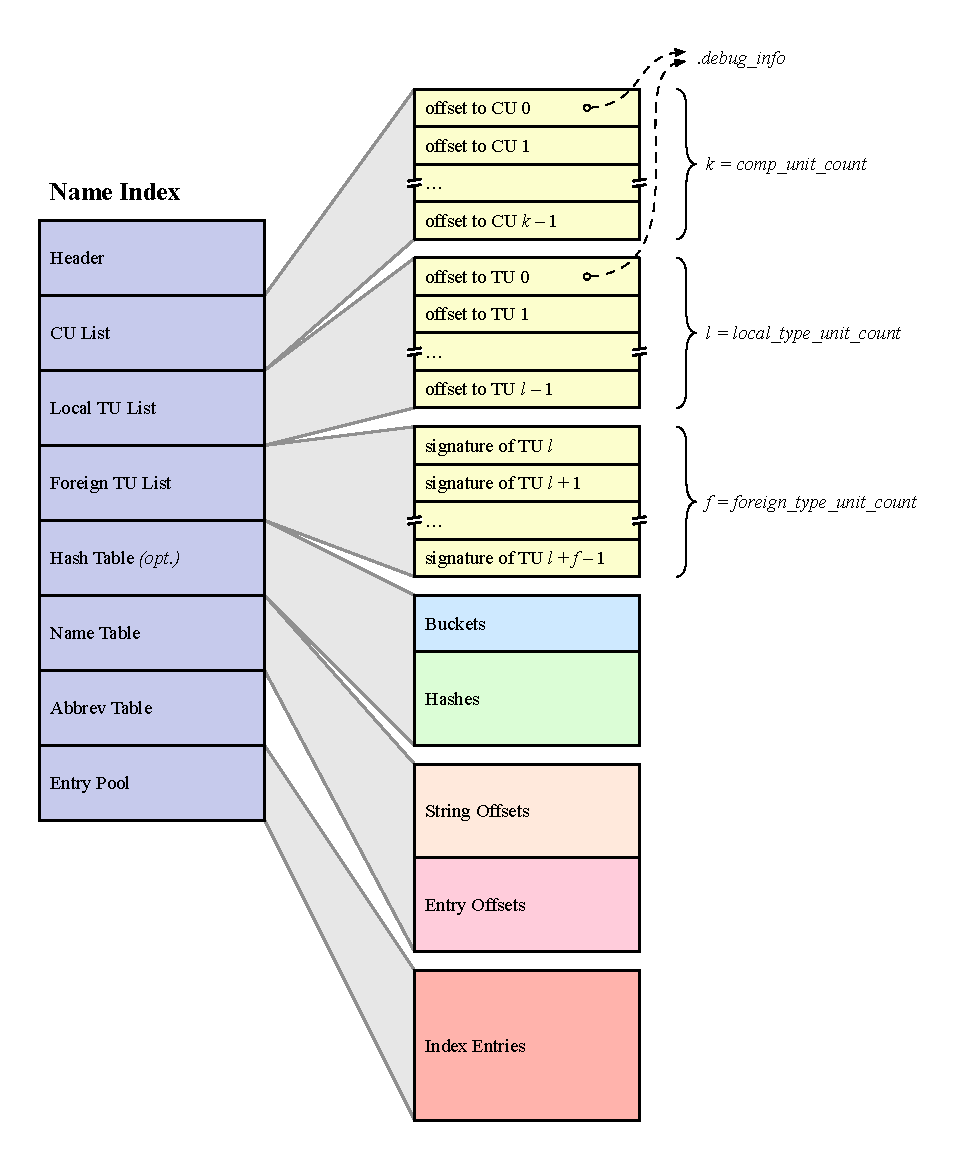
\includegraphics[keepaspectratio=true,scale=1.0]{name-index-drawings-6p1}

\begin{tikzpicture}[
  every node/.style={node font=\small, anchor=north west, text height=.8em, text depth=.2em, inner sep=4pt, outer ysep=0},
  caption/.style={node font=\small \bfseries, text width=90pt},
  overview/.style={draw, node font=\small, minimum height=28pt, text width=80pt},
  detail1/.style={draw, minimum height=14pt, text width=116pt},
  detail2/.style={draw, minimum height=28pt, text width=116pt},
  detail3/.style={draw, minimum height=38pt, text width=116pt},
  detail4/.style={draw, minimum height=72pt, text width=116pt},
  ellip/.style={draw, shape=broken rectangle, minimum height=14pt, text width=116pt},
  explode/.style={draw=black!50, fill=black!20, line join=bevel},
  header/.style={fill=headerblue},
  culist/.style={fill=cutuyellow},
  buckets/.style={fill=bucketsblue},
  hashes/.style={fill=hashesgreen},
  stroffsets/.style={fill=stroffsetspink},
  entryoffsets/.style={fill=entryoffsetspink},
  abbrevs/.style={fill=olive!40},
  indexentries/.style={fill=indexentriesorange}
]

% Name Table Overview

\begin{scope}[start chain=going below, node distance=0, yshift=-130pt]
  \node           [on chain,caption]  {Name Index};
  \node (header)  [on chain,overview,header] {Header};
  \node (culist)  [on chain,overview,header] {CU List};
  \node (ltulist) [on chain,overview,header] {Local TU List};
  \node (ftulist) [on chain,overview,header] {Foreign TU List};
  \node (hash)    [on chain,overview,header] {Hash Table};
  \node (names)   [on chain,overview,header] {Name Table};
  \node (abbrev)  [on chain,overview,header] {Abbrev Table};
  \node (pool)    [on chain,overview,header] {Entry Pool};
\end{scope}

% Exploded View of CU List

\begin{scope}[start chain=going below, node distance=0, shift={($(header.north east) + (72pt,130pt)$)}]
  \node (cu0) [on chain,detail1,culist] {offset to CU 0};
  \node (cu1) [on chain,detail1,culist] {offset to CU 1};
  \node (cu2) [on chain,ellip,culist]   {\dots};
  \node (cu3) [on chain,detail1,culist] {offset to CU $k - 1$};
\end{scope}

\begin{scope}[on background layer]
  \filldraw [explode] (culist.north east) -- (cu0.north west) -- (cu3.south west) -- (culist.south east) -- cycle;
\end{scope}

\path [decoration={brace,amplitude=6pt}] ([xshift=9pt]cu0.north east)
      [draw,decorate] -- ([xshift=9pt]cu3.south east)
      node [midway,right,inner xsep=9pt] {\texttt{comp\_unit\_count} $(= k)$};

% Exploded View of Local TU List

\begin{scope}[start chain=going below, node distance=0, shift={($(cu3.south west) + (0,-9pt)$)}]
  \node (ltu0) [on chain,detail1,culist] {offset to TU 0};
  \node (ltu1) [on chain,detail1,culist] {offset to TU 1};
  \node (ltu2) [on chain,ellip,culist]   {\dots};
  \node (ltu3) [on chain,detail1,culist] {offset to TU $t - 1$};
\end{scope}

\begin{scope}[on background layer]
  \filldraw [explode] (ltulist.north east) -- (ltu0.north west) -- (ltu3.south west) -- (ltulist.south east) -- cycle;
\end{scope}

\path [decoration={brace,amplitude=6pt}] ([xshift=9pt]ltu0.north east)
      [draw,decorate] -- ([xshift=9pt]ltu3.south east)
      node [midway,right,inner xsep=9pt] {\texttt{local\_type\_unit\_count} $(= t)$};

% Exploded View of Foreign TU List

\begin{scope}[start chain=going below, node distance=0, shift={($(ltu3.south west) + (0,-9pt)$)}]
  \node (ftu0) [on chain,detail1,culist] {signature of TU $t$};
  \node (ftu1) [on chain,detail1,culist] {signature of TU $t + 1$};
  \node (ftu2) [on chain,ellip,culist]   {\dots};
  \node (ftu3) [on chain,detail1,culist] {signature of TU $t + f - 1$};
\end{scope}

\begin{scope}[on background layer]
  \filldraw [explode] (ftulist.north east) -- (ftu0.north west) -- (ftu3.south west) -- (ftulist.south east) -- cycle;
\end{scope}

\path [decoration={brace,amplitude=6pt}] ([xshift=9pt]ftu0.north east)
      [draw,decorate] -- ([xshift=9pt]ftu3.south east)
      node [midway,right,inner xsep=9pt] {\texttt{foreign\_type\_unit\_count} $(= f)$};

% Exploded View of Hash Table

\begin{scope}[start chain=going below, node distance=0, shift={($(ftu3.south west) + (0,-9pt)$)}]
  \node (hash0) [on chain,detail2,buckets] {Buckets};
  \node (hash1) [on chain,detail3,hashes]  {Hashes};
\end{scope}

\begin{scope}[on background layer]
  \filldraw [explode] (hash.north east) -- (hash0.north west) -- (hash1.south west) -- (hash.south east) -- cycle;
\end{scope}

% Exploded View of Name Table

\begin{scope}[start chain=going below, node distance=0, shift={($(hash1.south west) + (0,-9pt)$)}]
  \node (name0) [on chain,detail3,stroffsets]   {String Offsets};
  \node (name1) [on chain,detail3,entryoffsets] {Entry Offsets};
\end{scope}

\begin{scope}[on background layer]
  \filldraw [explode] (names.north east) -- (name0.north west) -- (name1.south west) -- (names.south east) -- cycle;
\end{scope}

% Exploded View of Abbreviations

\begin{scope}[shift={($(name1.south west) + (0,-9pt)$)}]
  \node (abbrev0) [detail3,abbrevs] {Abbreviations};
\end{scope}

\begin{scope}[on background layer]
  \filldraw [explode] (abbrev.north east) -- (abbrev0.north west) -- (abbrev0.south west) -- (abbrev.south east) -- cycle;
\end{scope}

% Exploded View of Entry Pool

\begin{scope}[shift={($(abbrev0.south west) + (0,-9pt)$)}]
  \node (pool0) [detail3,indexentries] {Index Entries};
\end{scope}

\begin{scope}[on background layer]
  \filldraw [explode] (pool.north east) -- (pool0.north west) -- (pool0.south west) -- (pool.south east) -- cycle;
\end{scope}

%
\path [decoration={brace,amplitude=6pt}] ([xshift=9pt]hash0.north east)
      [draw,decorate] -- ([xshift=9pt]pool0.south east)
      node [midway,right,inner xsep=9pt] {\textit{see continued figure on the next pages}};

% Arrows pointing to .debug_info

\begin{scope}[shift={($(cu0.north east) + (15pt,27pt)$)}]
  \node (debuginfo) {\textit{.debug\_info}};
\end{scope}

\path ([xshift=28pt]cu0.center) coordinate (p1);
\path ([xshift=14pt]p1) coordinate (c1);
\path ([yshift=2pt]debuginfo.west) coordinate (p2);
\path ([xshift=-14pt]p2) coordinate (c2);
\draw [dashed,{Circle[open]}-{Stealth[]}] (p1) .. controls (c1) and (c2) .. (p2);

\path ([xshift=28pt]ltu0.center) coordinate (p3);
\path ([xshift=60pt]p3) coordinate (c3);
\path ([yshift=-2pt]debuginfo.west) coordinate (p4);
\path ([shift={(-21pt,-7pt)}]p4) coordinate (c4);
\draw [dashed,{Circle[open]}-{Stealth[]}] (p3) .. controls (c3) and (c4) .. (p4);

\end{tikzpicture}
\vspace{2mm}
\caption{Name Index Layout}
\label{fig:nameindexlayoutpart1}
\end{center}
\end{figure}

\begin{figure}[p]
\figurepart{2}{3}
\begin{center}
%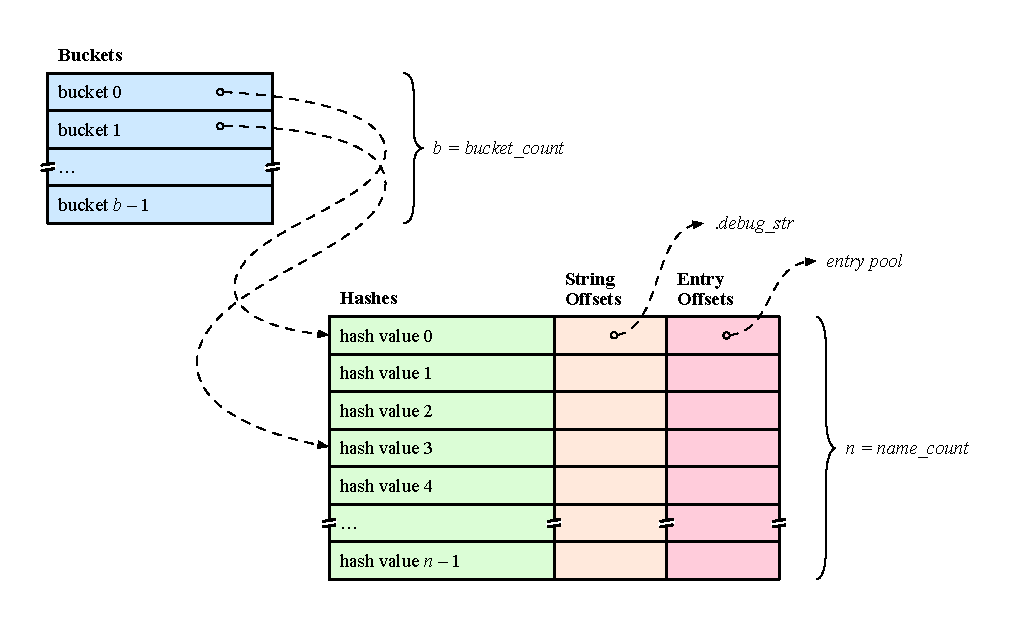
\includegraphics[keepaspectratio=true,scale=1.0]{name-index-drawings-6p2}

\begin{tikzpicture}[
  every node/.style={node font=\small, anchor=north west, text height=.8em, text depth=.2em, inner sep=4pt, outer ysep=0},
  % This diagram has a couple of two-line captions, so set the text depth
  % to make room for the second line.
  caption1/.style={node font=\small \bfseries, text depth=1.2em, text width=90pt},
  caption2/.style={node font=\small \bfseries, text depth=1.2em, text width=41pt},
  caption3/.style={node font=\small \bfseries, text depth=1.2em, text width=200pt},
  detail1/.style={draw, minimum height=14pt, text width=90pt},
  detail2/.style={draw, minimum height=14pt, text width=41pt},
  detail3/.style={draw, minimum height=14pt, text width=200pt},
  ellip1/.style={draw, shape=broken rectangle, minimum height=14pt, text width=90pt},
  ellip2/.style={draw, shape=broken rectangle, minimum height=14pt, text width=41pt},
  ellip3/.style={draw, shape=broken rectangle, minimum height=14pt, text width=200pt},
  buckets/.style={fill=bucketsblue},
  hashes/.style={fill=hashesgreen},
  stroffsets/.style={fill=stroffsetspink},
  abbreviations/.style={fill=olive!40},
  entryoffsets/.style={fill=entryoffsetspink}
]

% Buckets

\begin{scope}[start chain=going below, node distance=0]
  \node           [on chain,caption1]        {\\ Buckets};
  \node (bucket0) [on chain,detail1,buckets] {bucket 0};
  \node (bucket1) [on chain,detail1,buckets] {bucket 1};
  \node (bucket2) [on chain,ellip1,buckets]  {\dots};
  \node (bucket3) [on chain,detail1,buckets] {bucket $b - 1$};
\end{scope}

\path [decoration={brace,amplitude=6pt}] ([xshift=40pt]bucket0.north east)
      [draw,decorate] -- ([xshift=40pt]bucket3.south east)
          node [midway,right,inner xsep=9pt] {\texttt{bucket\_count} $(= b)$};

% Hashes

\begin{scope}[start chain=going below, node distance=0, shift={($(bucket3.south east) + (9pt,-24pt)$)}]
  \node (hashes) [on chain,caption1]       {\\ Hashes};
  \node (hash0)  [on chain,detail1,hashes] {hash value 1};
  \node (hash1)  [on chain,detail1,hashes] {hash value 2};
  \node (hash2)  [on chain,detail1,hashes] {hash value 3};
  \node (hash3)  [on chain,detail1,hashes] {hash value 4};
  \node (hash4)  [on chain,detail1,hashes] {hash value 5};
  \node (hash5)  [on chain,ellip1,hashes]  {\dots};
  \node (hash6)  [on chain,detail1,hashes] {hash value $n$};
\end{scope}

% String Offsets

\begin{scope}[start chain=going below, node distance=0, shift={($(hashes.north east) + (9pt, 0pt)$)}]
  \node (strs) [on chain,caption2]           {String \\ Offsets};
  \node (str0) [on chain,detail2,stroffsets] {};
  \node (str1) [on chain,detail2,stroffsets] {};
  \node (str2) [on chain,detail2,stroffsets] {};
  \node (str3) [on chain,detail2,stroffsets] {};
  \node (str4) [on chain,detail2,stroffsets] {};
  \node (str5) [on chain,ellip2,stroffsets]  {};
  \node (str6) [on chain,detail2,stroffsets] {};
\end{scope}

% Entry Offsets

\begin{scope}[start chain=going below, node distance=0, shift={($(strs.north east) + (9pt, 0pt)$)}]
  \node (entries) [on chain,caption2]             {Entry \\ Offsets};
  \node (entry0)  [on chain,detail2,entryoffsets] {};
  \node (entry1)  [on chain,detail2,entryoffsets] {};
  \node (entry2)  [on chain,detail2,entryoffsets] {};
  \node (entry3)  [on chain,detail2,entryoffsets] {};
  \node (entry4)  [on chain,detail2,entryoffsets] {};
  \node (entry5)  [on chain,ellip2,entryoffsets]  {};
  \node (entry6)  [on chain,detail2,entryoffsets] {};
\end{scope}

\path [decoration={brace,amplitude=6pt}] ([xshift=9pt]entry0.north east)
      [draw,decorate] -- ([xshift=9pt]entry6.south east)
      node [midway,right,inner xsep=9pt] {\begin{tabular}{c}
                                          \texttt{name\_count} \\
                                                     $(= n)$
                                          \end{tabular}};

% Arrows pointing to .debug_str and entry pool

\path (str0.center) coordinate (p1);
\path ([xshift=18pt]p1) coordinate (c1);
\path ([shift={(36pt,45pt)}]p1) coordinate (p2);
\path ([xshift=-18pt]p2) coordinate (c2);
\draw [dashed,{Circle[open]}-{Stealth[]}] (p1) .. controls (c1) and (c2) .. (p2) node [anchor=west]
																					{$.debug\_str$};

\path (entry0.center) coordinate (p3);
\path ([xshift=18pt]p3) coordinate (c3);
\path ([shift={(36pt,27pt)}]p3) coordinate (p4);
\path ([xshift=-18pt]p4) coordinate (c4);
\draw [dashed,{Circle[open]}-{Stealth[]}] (p3) .. controls (c3) and (c4) .. (p4) node [anchor=west]
																					{$index\ entries$};

% Arrows from buckets to hashes

\path ([xshift=24pt]bucket0.center) coordinate (p5);
\path ([xshift=130pt]p5) coordinate (c5);
\path ([xshift=-70pt]hash0.west) coordinate (c6);
\draw [dashed,{Circle[open]}-{Stealth[]}] (p5) .. controls (c5) and (c6) .. (hash0.west);

\path ([xshift=24pt]bucket1.center) coordinate (p7);
\path ([xshift=120pt]p7) coordinate (c7);
\path ([xshift=-144pt]hash3.west) coordinate (c8);
\draw [dashed,{Circle[open]}-{Stealth[]}] (p7) .. controls (c7) and (c8) .. (hash3.west);

% Abbreviations

\begin{scope}[start chain=going below, node distance=0, shift={($(hash6.south west) + (-48pt,-24pt)$)}]
  \node (abbreves)[on chain,caption3]              {\\ Abbreviations};
  \node (abbrev1) [on chain,detail3,abbreviations] {abbrev code $m$};
  \node (abbrev2) [on chain,detail3,abbreviations] {tag (DW\_TAG)};
  \node (abbrev3) [on chain,detail3,abbreviations] {idx attrib name (DW\_IDX), form (DW\_FORM)};
  \node (abbrev4) [on chain,ellip3,abbreviations]  {\dots};
  \node (abbrev5) [on chain,detail3,abbreviations] {idx attrib name (DW\_IDX), form (DW\_FORM)};
  \node (abbrev6) [on chain,detail3,abbreviations] {0, 0 (end of abbrev code $m$)};
  \node (abbrev7) [on chain,ellip3,abbreviations]  {\dots};
  \node (abbrev8) [on chain,detail3,abbreviations] {0 (end of abbreviations)};
  \node (abbrev9) [on chain,detail3,abbreviations] {\textit{padding}};
\end{scope}

\path [decoration={brace,amplitude=6pt}] ([xshift=9pt]abbrev1.north east)
      [draw,decorate] -- ([xshift=9pt]abbrev9.south east)
      node [midway,right,inner xsep=9pt] {\begin{tabular}{c}
                                          \texttt{abbrev\_table\_size} \\
                                                     $(= s)$
                                          \end{tabular}};

\end{tikzpicture}

\vspace{5mm}
%\caption{Name Index Layout \textit{(continued)}}
Figure~\ref{fig:nameindexlayoutpart1}: Name Index Layout \textit{(continued)}
%\label{fig:nameindexlayoutpart2}
\end{center}
\end{figure}

\begin{figure}[t]
\figurepart{3}{3}
\begin{center}
%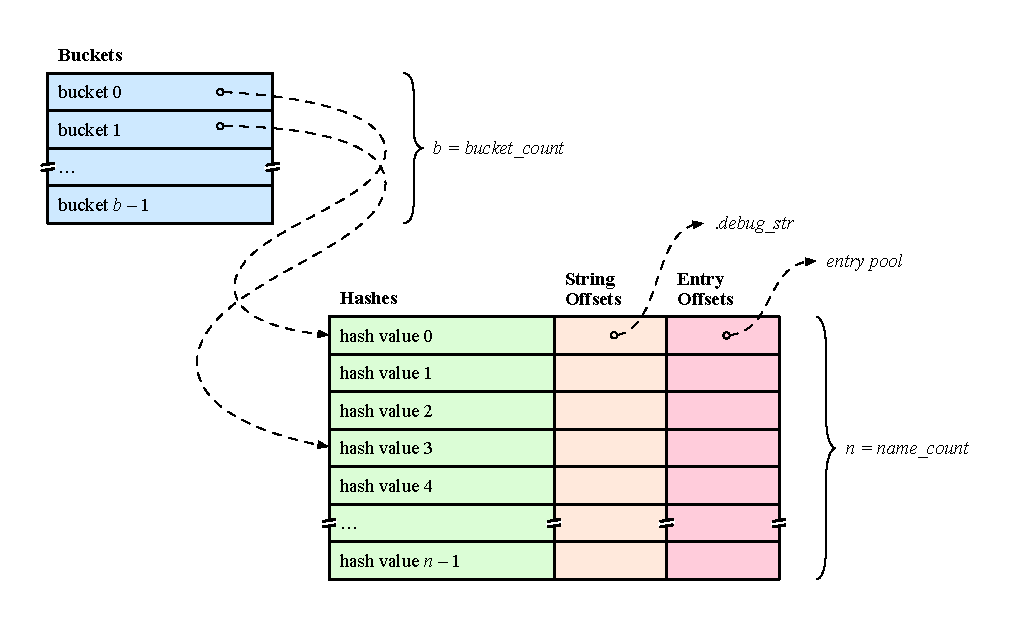
\includegraphics[keepaspectratio=true,scale=1.0]{name-index-drawings-6p2}

%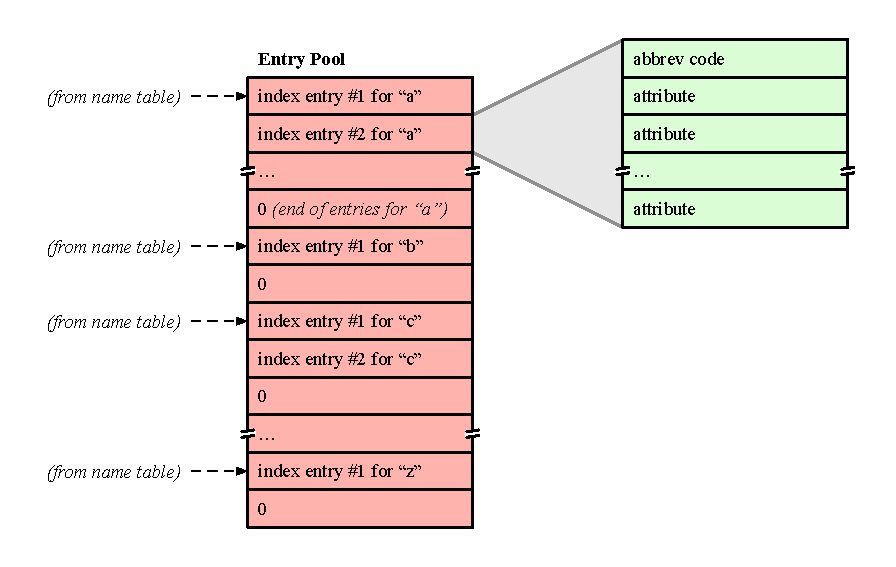
\includegraphics[keepaspectratio=true,scale=1.0]{name-index-drawings-6p3}
\begin{tikzpicture}[
  every node/.style={node font=\small, anchor=north west, text height=.8em, text depth=.2em,
             inner sep=4pt, outer ysep=0},
  caption/.style={node font=\small \bfseries, text width=120pt},
  detail/.style={draw, node font=\small, minimum height=14pt, text width=120pt},
  ellip/.style={draw, shape=broken rectangle, minimum height=14pt, text width=120pt},
  explode/.style={draw=black!50, fill=black!20, line join=bevel},
  indexentries/.style={fill=indexentriesorange}
]

% Index Entries

\begin{scope}[start chain=going below, node distance=0]
  \node           [on chain,caption]             {Index Entries};
  \node (entry0)  [on chain,detail,indexentries] {index entry \#1 for ``a''};
  \node (entry1)  [on chain,detail,indexentries] {index entry \#2 for ``a''};
  \node (entry2)  [on chain,ellip,indexentries]  {\dots};
  \node (entry3)  [on chain,detail,indexentries] {0 \textit{(end of entries for ``a'')}};
  \node (entry4)  [on chain,detail,indexentries] {index entry \#1 for ``b''};
  \node (entry5)  [on chain,detail,indexentries] {index entry \#2 for ``b''};
  \node (entry6)  [on chain,ellip,indexentries]  {\dots};
  \node (entry7)  [on chain,detail,indexentries] {0 \textit{(end of entries for ``b'')}};
  \node (entry8)  [on chain,detail,indexentries] {index entry \#1 for ``c''};
  \node (entry9)  [on chain,ellip,indexentries]  {\dots};
\end{scope}

% Exploded Index Entry

\begin{scope}[start chain=going below, node distance=0, shift={($(entry1.north east) + (50pt,30pt)$)}]
  \node (abbrev) [on chain,detail,indexentries] {abbrev code $m$};
  \node (attr1)  [on chain,detail,indexentries] {idx attrib value};
  \node (attr2)  [on chain,detail,indexentries] {idx attrib value};
  \node (attr3)  [on chain,ellip,indexentries]  {\dots};
  \node (attr4)  [on chain,detail,indexentries] {idx attrib value};
\end{scope}

\begin{scope}[on background layer]
  \filldraw [explode] (entry1.north east) -- (abbrev.north west) -- (attr4.south west) -- (entry1.south east) -- cycle;
\end{scope}

% Arrows

\node (from1) [anchor=east] at ([xshift=-30pt]entry0.west) {\begin{tabular}{c}
															\textit{from entry offsets} \\
															\textit{of name table}
															\end{tabular} };
\draw [dashed,-{Stealth[]}] (from1) -- (entry0.west);

\node (from2) [anchor=east] at ([xshift=-30pt]entry4.west) {\begin{tabular}{c}
															\textit{from entry offsets} \\
															\textit{of name table}
															\end{tabular} };
\draw [dashed,-{Stealth[]}] (from2) -- (entry4.west);

\node (from2) [anchor=east] at ([xshift=-30pt]entry8.west) {\begin{tabular}{c}
															\textit{from entry offsets} \\
															\textit{of name table}
															\end{tabular} };
\draw [dashed,-{Stealth[]}] (from2) -- (entry8.west);

\end{tikzpicture}

\vspace{5mm}
%\caption{Name Index Layout \textit{(concluded)}}
Figure~\ref{fig:nameindexlayoutpart1}: Name Index Layout \textit{(concluded)}
%\label{fig:nameindexlayoutpart3}
\end{center}
\end{figure}

The formats of the header and the hash lookup table are described
in Section \refersec{chap:datarepresentationofthenameindex}.

The list of CUs and the list of local TUs are each an array of
offsets, each of which is the offset of a compile unit or a type unit
in the \dotdebuginfo{} section. For a per-CU index, there is a single CU
entry, and there may be a TU entry for each type unit generated in the
same translation unit as the single CU. For a per-module index, there
will be one CU entry for each compile unit in the module, and one TU
entry for each unique type unit in the module. Each list is indexed
starting at 0.

The list of foreign TUs is an array of 64-bit (\DWFORMrefsigeight) type
signatures, representing types referenced by the index whose
definitions have been placed in a different object file (that is, a split
DWARF object). This list may be empty.
The foreign TU list immediately follows the local TU list
and they both use the same index, so that if there are $N$ local TU entries,
the index for the first foreign TU is $N$.

The name table is logically a table with a row for each unique name in
the index, and two columns. The first column contains a reference to
the name, as a string. The second column contains the offset within
the entry pool of the list of index entries for the name.

\needlines{4}
The abbreviations table describes the formats of the entries in the
entry pool. Like the DWARF abbreviations table in the \dotdebugabbrev{}
section, it defines one or more abbreviation codes. Each abbreviation
code provides a DWARF tag value followed by a list of pairs that
defines an attribute and form code used by entries with that
abbreviation code.

The entry pool contains all the index entries, grouped by name. The
second column of the name list points to the first index entry for the
name, and all the index entries for that name are placed one after the
other.

Each index entry begins with an unsigned LEB128 abbreviation code.
The  abbreviation list for that code provides the DWARF tag value for
the entry as well as the set of attributes provided by the entry and
their forms.

\needlines{4}
The standard
\bb
\addtoindex{index attribute}s (see Table \refersec{tab:indexattributeencodings})
\eb
are:
\begin{itemize}
\item Compilation Unit (CU), a reference to an entry in the list of
    CUs. In a per-CU index, index entries without this
\bb
	index attribute
\eb
    implicitly refer to the single CU.

\item Type Unit (TU), a reference to an entry in the list of local
    or foreign TUs.

\item Debugging information entry offset within the CU or TU.

\item Parent debugging information entry,
    a reference to the index entry for the parent.
    This is represented as the offset of the entry relative to
    the start of the entry pool.

\item Type hash, an 8-byte hash of the type declaration.

\end{itemize}

\needlines{6}
It is possible that an indexed debugging information entry
has a parent that is not
indexed (for example, if its parent does not have a name attribute).
In such a case, a parent
\bb
index attribute
\eb
may point to a nameless index
entry (that is, one that cannot be reached from any entry in the
name table), or it may point to the nearest ancestor that does
have an index entry.

A producer may define additional
\bb
producer-specific
index attributes,
\eb
and a consumer will be able to ignore and skip over any
\bb
index attributes
\eb
it is not prepared to handle.

\needlines{4}
When an index entry refers to a foreign type unit, it may have
\bb
index attributes
\eb
for both CU and (foreign) TU. For such entries, the CU
\bb
index attribute
\eb
gives the consumer a reference to the CU that may be used to
locate a \splitDWARFobjectfile{} that contains the type unit.

\textit{The type hash
\bb
index attribute,
\eb
not to be confused with the type signature
for a TU, may be provided for type entries whose declarations are not
in a type unit, for the convenience of link-time or post-link
utilities that wish to de-duplicate type declarations across
compilation units. The type hash, however, is computed by the
same method as specified for type signatures.}

The last entry for each name is followed by a zero byte that
terminates the list. There may be gaps between the lists.

\subsubsection{Per-CU versus Per-Module Indexes}
\label{chap:percuvspermoduleindexes}
\textit{In a per-CU index, the CU list may have only a single entry,
and index entries may omit the CU
\bb
attribute.
\eb
(Cross-module or link-time
optimization, however, may produce an object file with several compile
units in one object. A compiler in this case may produce a separate
index for each CU, or a combined index for all CUs. In the latter
case, index entries will require the CU
\bb
attribute.)
\eb
Most name table
entries may have only a single index entry for each, but sometimes a
name may be used in more than one context and will require multiple
index entries, each pointing to a different debugging information
entry.}

\textit{When linking object files containing per-CU indexes, the
linker may choose to concatenate the indexes as ordinary sections,
or it may choose to combine the input indexes into a single
per-module index.}

\textit{A per-module index will contain a number of CUs, and each index
entry contains a CU attribute or a TU attribute to identify which
CU or TU contains the debugging information entry being indexed. When a
given name is used in multiple CUs or TUs, it will typically have a
series of index entries pointing to each CU or TU where it is declared.
For example, an index entry for a \addtoindex{C++} namespace needs to
list each occurrence, since each CU may contribute additional names to
the namespace, and the consumer needs to find them all. On the
other hand, some index entries do not need to list more than one
definition; for example, with the one-definition rule in \addtoindex{C++},
duplicate entries for a function may be omitted, since the consumer
only needs to find one declaration. Likewise, a per-module index needs
to list only a single copy of a type declaration contained in a type
unit.}

\needlines{4}
\textit{For the benefit of link-time or post-link utilities that consume
per-CU indexes and produce a per-module index, the per-CU index
entries provide the tag encoding for the original debugging
information entry, and may provide a type hash for certain types that
may benefit from de-duplication. For example, the standard declaration
of the typedef \texttt{uint32\_t} is likely to occur in many CUs, but a
combined per-module index needs to retain only one; a user declaration
of a typedef \texttt{mytype} may refer to a different type at each
occurrence, and a combined per-module index retains each unique
declaration of that type.}


\subsubsection{Data Representation of the Name Index}
\label{chap:datarepresentationofthenameindex}
The name index is placed in a section named \dotdebugnames, and
consists of the eight parts described in the following sections.

\subsubsubsection{Section Header}
\label{chap:sectionheader}
The section header contains the following fields:
\begin{enumerate}[1. ]

\item \HFNunitlength{} (\livelink{datarep:initiallengthvalues}{initial length}) \\
The length of this contribution to the name index section,
not including the length field itself
\bb
(see Section \refersec{datarep:initiallengthvalues}).
\eb


\item \HFNversion{} (\HFTuhalf) \\
A version number\addtoindexx{version number!name index table}
(see Section \refersec{datarep:nameindextable}).
This number is specific to the name index table and is
independent of the DWARF version number.

\item \HFNpadding{} (\HFTuhalf) \\
Reserved to DWARF (must be zero).

\item \HFNcompunitcount{} (\HFTuword) \\
The number of CUs in the CU list.

\item \HFNlocaltypeunitcount{} (\HFTuword) \\
The number of TUs in the local TU list.

\item \HFNforeigntypeunitcount{} (\HFTuword) \\
The number of TUs in the foreign TU list.

\item \HFNbucketcount{} (\HFTuword) \\
The number of hash buckets in the hash lookup table.
If there is no hash lookup table, this field contains 0.

\item \HFNnamecount{} (\HFTuword) \\
The number of unique names in the index.

\item \HFNabbrevtablesize{} (\HFTuword) \\
The size in bytes of the abbreviations table.

\item
\bb
\HFNaugmentationsize{} (\HFTuword) \\
The size in bytes of the augmentation sequence.
This value must be a multiple of four.
\eb

\item
\bbeb
\HFNaugmentation{} (sequence of \HFTubyte) \\
\addtoindexx{augmentation sequence}
\bb
A producer-specific
sequence of bytes,
\eb
which provides additional information about the contents of
this index. If provided, the sequence begins with
\bb
four bytes which serve as a producer ID.
\eb
The remainder of the
\bb
sequence
\eb
is meant to be read by a cooperating consumer, and its
contents and interpretation are not specified here. The
\bb
block is padded with zero bytes
\eb
to a multiple of four bytes in length.

\textit{The presence of an unrecognized augmentation
\bb
producer ID
\eb
does not make it
impossible for a consumer to process data in the \dotdebugnames{} section.
The augmentation
\db
sequence only provides hints to the consumer regarding
the completeness of the set of names in the index.}

\end{enumerate}

\needlines{4}
\subsubsubsection{List of CUs}
The list of CUs immediately follows the header. Each entry in the
list is an offset of the corresponding compilation unit
in the \dotdebuginfo{} section.
In the DWARF-32 format, a section offset is 4 bytes,
while in the DWARF-64 format, a section offset is 8 bytes.

The total number of entries in the list is given by \texttt{comp\_unit\_count}.
There must be at least one CU.

\needlines{4}
\subsubsubsection{List of Local TUs}
The list of local TUs immediately follows the list of CUs. Each
entry in the list is an offset of the corresponding type unit
in the \dotdebuginfo{} section.
In the DWARF-32 format, a section offset is 4 bytes,
while in the DWARF-64 format, a section offset is 8 bytes.

\bb
Any local TU entry with a maximum representable value is
considered not present. Any index entry referencing such
a local TU entry should be ignored.
\eb

The total number of entries in the list is given by
\HFNlocaltypeunitcount{}. This list may be empty.

\subsubsubsection{List of Foreign TUs}
The list of foreign TUs immediately follows the list of local TUs.
Each entry in the list is a 8-byte type signature (as described by
\DWFORMrefsigeight).

The number of entries in the list is given by \HFNforeigntypeunitcount{}.
This list may be empty.

\needlines{4}
\subsubsubsection{Hash Lookup Table}
The optional hash lookup table immediately follows the list of type signatures.

The hash lookup table is actually two separate arrays: an array of
buckets, followed immediately by an array of hashes. The number of
entries in the buckets array is given by \HFNbucketcount{}, and the number
of entries in the hashes array is given by \HFNnamecount{}. Each array
contains 4-byte unsigned integers.

\needlines{4}
Symbols are entered into the hash table by first computing a hash
value from the symbol name. The hash is computed
using the "DJB" hash function\addtoindexx{DJB hash function}
described in Section \refersec{datarep:nametablehashfunction}.
Given a hash value for the symbol,
the symbol is entered into a bucket whose index is the hash value
modulo \HFNbucketcount{}. The buckets array is indexed starting at 0.

For the purposes of the hash computation, each symbol name should be
folded according to the simple case folding algorithm defined in the
"Caseless Matching" subsection of Section 5.18 ("Case Mappings") of
the \addtoindex{Unicode} Standard, Version 9.0.0. The original symbol
name, as it appears in the source code, should be stored in the name
table.\addtoindexx{name index!case folding}\db

\textit{Thus, two symbols that differ only by case will hash to
the same slot, but the consumer will be able to distinguish the names
when appropriate.}

\needlines{6}
The simple case folding algorithm is further described
in the CaseFolding.txt file distributed with the \addtoindex{Unicode}
Character Database. That file defines four classes of mappings:
Common (C), Simple (S), Full (F), and Turkish (T).
The hash computation specified here uses the C + S mappings only,
which do not affect the total length of the string, with the addition
that Turkish upper case dotted '\.{I}' and lower case dotless '\i'
are folded to the Latin lower case 'i'.

Each bucket contains the index of an entry in the hashes array. The
hashes array is indexed starting at 1, and an empty bucket is
represented by the value 0.

\needlines{4}
The hashes array contains a sequence of the full hash values for each
symbol. All symbols that have the same index into the bucket list
follow one another in the hashes array, and the indexed entry in
the bucket list refers to the first symbol.
When searching for a symbol, the search
starts at the index given by the bucket, and continues either until a
matching symbol is found or until a hash value from a different bucket
is found. If two different symbol names produce the same hash value,
that hash value will occur twice in the hashes array. Thus, if a
matching hash value is found, but the name does not match, the search
continues visiting subsequent entries in the hashes table.

When a matching hash value is found in the hashes array, the index of
that entry in the hashes array is used to find the corresponding entry
in the name table.

\needlines{6}
\subsubsubsection{Name Table}
\label{chap:nametable}
The name table immediately follows the hash lookup table. It
consists of two arrays: an array of string offsets, followed
immediately by an array of entry offsets. The items in both
arrays are section offsets: 4-byte unsigned integers for the
DWARF-32 format or 8-byte unsigned integers for the DWARF-64
format. The string offsets in the first array refer to names in
the \dotdebugstr{} (or \dotdebugstrdwo) section. The entry offsets
in the second array refer to index entries, and are relative to
the start of the entry pool area.

These two arrays are indexed starting at 1, and correspond
one-to-one with each other. The length of each array is
given by \HFNnamecount{}.

If there is a hash lookup table, the hashes array corresponds on
a one-to-one basis with the string offsets array and with the
entry offsets array.

\textit{If there is no hash lookup table, there is no ordering
requirement for the name table.}

\needlines{6}
\subsubsubsection{Abbreviations Table}
The abbreviations table immediately follows the name table. This table
consists of a series of abbreviation declarations. Its size is given
by \HFNabbrevtablesize{}.

Each abbreviation declaration defines the tag and other attributes for
a particular form of index entry. Each declaration starts with an
unsigned LEB128 number representing the abbreviation code itself. It
is this code that appears at the beginning of an index entry. The
abbreviation code must not be 0.

The abbreviation code is followed by another unsigned LEB128 number
that encodes the tag of the debugging information entry corresponding
to the index entry.

Following the tag encoding is a series of attribute specifications.
Each
\bb
index attribute
\eb
consists of two parts: an unsigned LEB128 number that
represents the index attribute, and another unsigned LEB128 number
that represents the
\bb
index attribute's
\eb
form (as described in
Section \refersec{datarep:attributeencodings}). The series of attribute
specifications ends with an entry containing 0 for the attribute and
0 for the form.

The index attributes and their meanings are listed in
Table \refersec{tab:indexattributeencodings}.

\needlines{10}
\begin{centering}
\setlength{\extrarowheight}{0.1cm}
\begin{longtable}{l|P{7cm}}
  \caption{Index attribute encodings} \label{tab:indexattributeencodings}\\
  \hline \bbeb \bfseries Index attribute name & \bfseries Meaning \\ \hline
\endfirsthead
  \bbeb \bfseries Index attribute name & \bfseries Meaning \\ \hline
\endhead
  \hline \emph{Continued on next page}
\endfoot
  \hline
\endlastfoot
\DWIDXcompileunitTARG 	& Index of CU                                  \\
\DWIDXtypeunitTARG    	& Index of TU (\mbox{local} or foreign)        \\
\DWIDXdieoffsetTARG   	& Offset of DIE within CU or TU                \\
\DWIDXparentTARG      	& Index of name \mbox{table} entry for parent  \\
\DWIDXtypehashTARG    	& Hash of type \mbox{declaration}              \\
\bb
\DWIDXexternalTARG		& Whether \DWATexternal{} is present
						  on the declaration (flag)
\eb \\
\end{longtable}
\end{centering}

The abbreviations table ends with an entry consisting of a single 0
byte for the abbreviation code. The size of the table given by
\HFNabbrevtablesize{} may include optional padding following the
terminating 0 byte.

\needlines{4}
\subsubsubsection{Entry Pool}
The entry pool immediately follows the abbreviations table.
Each entry in the entry offsets array in the name table (see
Section \ref{chap:nametable})
points to an offset in the entry pool, where a series
of index entries for that name is located.

\needlines{4}
Each index entry in the series begins with an abbreviation code, and is
followed by the
\bb
index attribute values
\eb
described by the abbreviation declaration
for that code. The last index entry in the series is followed by a
terminating entry whose abbreviation code is 0.

\bb
Each index entry has a flag indicating whether the corresponding DIE
has the \DWATexternal{} attribute with a true value. If the
\DWIDXexternal{} attribute is missing from an entry, it means that
\DWATexternal{} is false for that DIE.
\eb

Gaps are not allowed between entries in a series (that is, the entries
for a single name must all be contiguous), but there may be gaps
between series.

\textit{For example, a producer/consumer combination may find
it useful to maintain alignment.}

The size of the entry pool is the remaining size of the contribution to
the index section, as defined by the \texttt{unit\_length} header field.

\needlines{6}
\subsection{Lookup by Address}
\label{chap:lookupbyaddress}
For \addtoindexx{lookup!by address}
lookup by address, a table is maintained in a separate
\addtoindexx{accelerated access!by address}
object file section called
\dotdebugaranges{}. The table consists
of sets of variable length entries, each set describing the
portion of the program\textquoteright{}s address space that is covered by
a single compilation unit.

\needlines{4}
Each set begins with a header containing five values:
\begin{enumerate}[1. ]
\item \HFNunitlength{} (\livelink{datarep:initiallengthvalues}{initial length}) \\
The length of this contribution to the address lookup section,
not including the length field itself
\bb
(see Section \refersec{datarep:initiallengthvalues}).
\eb

\item \HFNversion{} (\HFTuhalf) \\
A version number\addtoindexx{version number!address lookup table}
(see Section \refersec{datarep:addrssrangetable}).
This number is specific to the address lookup table and is
independent of the DWARF version number.

\item \HFNdebuginfooffset{} (section offset) \\
The offset from the
\addtoindexx{section offset!in .debug\_aranges header}
beginning of the \dotdebuginfo{} section of the
compilation unit header referenced by the set.

\item \HFNaddresssize{} (\HFTubyte) \\
The \addtoindex{size of an address}
in bytes on the target architecture.
\db

\item \HFNreservedwassegmentselectorsize{}
\bbeb
\\

\end{enumerate}

\needlines{6}
This header is followed by a variable number of address range
descriptors. Each descriptor is a
\bb
pair consisting of the beginning address
\eb
of a range of text or data covered by some entry owned by
the corresponding compilation unit, followed by the
\db
length of that range. A particular set is terminated by an
entry consisting of
\bb
two
\eb
zeroes.
\db
By scanning the table, a debugger can quickly decide
which compilation unit to look in to find the debugging
information for an object that has a given address.

\bb
A range description entry whose address is the reserved address (see
Section \refersec{chap:reservedtargetaddress}), indicates a
non-existent range, which is equivalent to
omitting the range description.
\eb

\textit{If the range of addresses covered by the text and/or data
of a compilation unit is not contiguous, then there may be
multiple address range descriptors for that compilation unit.}


\section{Line Number Information}
\label{chap:linenumberinformation}
\textit{A source\dash level debugger needs to know how to
\addtoindexx{line number information|see{\textit{also} statement list attribute}}
associate locations in the source files with the corresponding
machine instruction addresses in the executable or the shared
object files used by that executable object file. Such an
association makes it possible for the debugger user
to specify machine instruction addresses in terms of source
locations. This is done by specifying the line number
and the source file containing the statement. The debugger
can also use this information to display locations in terms
of the source files and to single step from line to line,
or statement to statement.}

Line number information generated for a compilation unit is
represented in the
\dotdebugline{} section of an object file, and optionally
also in the \dotdebuglinestr{} section, and
is referenced by a corresponding compilation unit debugging
information entry
(see Section \refersec{chap:fullandpartialcompilationunitentries})
in the \dotdebuginfo{} section.

\textit{Some computer architectures employ more than one instruction
set (for example, the ARM
\addtoindexx{ARM instruction set architecture}
and
MIPS architectures support
\addtoindexx{MIPS instruction set architecture}
a 32-bit as well as a 16-bit instruction set). Because the
instruction set is a function of the program counter, it is
convenient to encode the applicable instruction set in the
\dotdebugline{} section as well.}

\textit{If space were not a consideration, the information provided
in the \dotdebugline{}
section could be represented as a large
matrix, with one row for each instruction in the emitted
object code. The matrix would have columns for:}
\begin{itemize}
\item \textit{the source file name}
\item \textit{the source line number}
\item \textit{the source column number}
\item \textit{whether this instruction is the beginning of a source statement}
\item \textit{whether this instruction is the beginning of a \addtoindex{basic block}}
\item \textit{and so on}
\end{itemize}
\textit{Such a matrix, however, would be impractically large. We
shrink it with two techniques. First, we delete from
the matrix each row whose file, line, source column and
discriminator\addttindexx{discriminator}
is identical with that of its
predecessors. Any deleted row would never be the beginning of
a source statement. Second, we design a byte-coded language
for a state machine and store a stream of bytes in the object
file instead of the matrix. This language can be much more
compact than the matrix. To the line number information a
consumer must \doublequote{run} the state machine
to generate the matrix for each compilation unit of interest.
The concept of an encoded matrix also leaves
room for expansion. In the future, columns can be added to the
matrix to encode other things that are related to individual
instruction addresses.}

\needlines{10}
\subsection{Definitions}
\label{chap:definitions}
The following terms are used in the description of the line
number information format:

\begin{longtable} {lP{9cm}}
state machine &
The hypothetical machine used by a consumer of the line number
information to expand the byte\dash coded
instruction stream into a matrix of
line number information. \\

line number program &
A series of byte\dash coded
line number information instructions representing
one compilation unit. \\

\addtoindex{basic block} &
 A sequence of instructions where only the first instruction may be a
branch target and only the last instruction may transfer control. A
subprogram invocation is defined to be an exit from a
\addtoindex{basic block}.

\textit{A \addtoindex{basic block} does not
necessarily correspond to a specific source code
construct.} \\

sequence &
A series of contiguous target machine instructions. One compilation unit
may emit multiple sequences (that is, not all instructions within a
compilation unit are assumed to be contiguous). \\
\end{longtable}

\needlines{8}
\subsection{State Machine Registers}
\label{chap:statemachineregisters}
The line number information state machine has a number of
registers as shown in Table \referfol{tab:statemachineregisters}.

\begin{longtable}{l|P{10cm}}
  \caption{State machine registers } \label{tab:statemachineregisters} \\
  \hline \bfseries Register name&\bfseries Meaning\\ \hline
\endfirsthead
  \bfseries Register name&\bfseries Meaning\\ \hline
\endhead
  \hline
  \multicolumn{2}{l}{\emph{Continued on next page}}
\endfoot
  \hline
\endlastfoot
\addtoindexi{\texttt{address}}{address register!in line number machine}&
The program\dash counter value corresponding to a machine instruction
generated by the compiler. \\

\addttindex{op\_index} &
An unsigned integer representing the index of an operation within a VLIW
instruction. The index of the first operation is 0. For non-VLIW
architectures, this register will always be 0.  \\

\addttindex{file} &
An unsigned integer indicating the identity of the source file
corresponding to a machine instruction.
\bb
Files are numbered beginning at 0.
\eb
\\

\addttindex{line} &
An unsigned integer indicating a source line number. Lines are numbered
beginning at 1. The compiler may emit the value 0 in cases where an
instruction cannot be attributed to any source line. \\

\addttindex{column} &
An unsigned integer indicating a column number within a source line.
Columns are numbered beginning at 1. The value 0 is reserved to indicate
that a statement begins at the \doublequote{left edge} of the line. \\

\addttindex{is\_stmt} &
A boolean indicating that the current instruction is a recommended
breakpoint location. A recommended breakpoint location
is intended to \doublequote{represent} a line, a
statement and/or a semantically distinct subpart of a
statement. \\

\addttindex{basic\_block}  &
A boolean indicating that the current instruction is the beginning of a
\addtoindex{basic block}. \\

\addttindex{end\_sequence} &
A boolean indicating that the current address is that of the first byte after
the end of a sequence of target machine instructions.
\addttindex{end\_sequence}
terminates a sequence of lines; therefore other information in the same
row is not meaningful. \\

\addttindex{prologue\_end} &
A boolean indicating that the current address is one (of possibly many)
where execution should be suspended for a breakpoint at the entry of a
function. \\

\addttindex{epilogue\_begin} &
A boolean indicating that the current address is one (of possibly many)
where execution should be suspended for a breakpoint just prior to
the exit of a function. \\

\bb
\addttindex{prologue\_epilogue} &
A boolean indicating that the current row describes instructions
within a prologue or epilogue range.
\eb
\\

\addttindex{isa} &
An unsigned integer whose value encodes the applicable
instruction set architecture for the current instruction.

\textit{The encoding of instruction sets should be shared by all
users of a given architecture. It is recommended that this
encoding be defined by the ABI authoring committee for each
architecture.} \\

\addttindex{discriminator} &
An unsigned integer identifying the block to which the
current instruction belongs. Discriminator values are assigned
arbitrarily by the DWARF producer and serve to distinguish
among multiple blocks that may all be associated with the
same source file, line, and column. Where only one block
exists for a given source position, the discriminator value
is
\db
zero. \\
\end{longtable}

The \texttt{address} and \addttindex{op\_index} registers,
taken together, form an \addtoindex{operation pointer} that can
reference any individual operation within the instruction stream.

At the beginning  of each sequence within a line number
program, the state of the registers is as show in Table
\refersec{tab:linenumberprograminitiastate}.

\begin{table}[h]
\caption{Line number program initial state}
\label{tab:linenumberprograminitiastate}
\begin{center}
\begin{tabular}{l|p{9.5cm}}
\hline
\texttt{address} & 0 \\
\addttindex{op\_index} & 0 \\
\bbeb
\texttt{file} & 0 \\
\texttt{line} & 1 \\
\texttt{column} & 0 \\
\addttindex{is\_stmt} & determined by \addttindex{default\_is\_stmt}
			in the line number program header \\
\addttindex{basic\_block}    & \doublequote{false} \addtoindexx{basic block} \\
\addttindex{end\_sequence}   & \doublequote{false} \\
\addttindex{prologue\_end}   & \doublequote{false} \\
\addttindex{epilogue\_begin} & \doublequote{false} \\
\bbeb
\addttindex{prologue\_epilogue} & \doublequote{false} \\
\addttindex{isa} & 0 \\
\addttindex{discriminator} & 0 \\
\hline
\end{tabular}
\end{center}
\vspace{5mm}
\end{table}

\textit{The
\addttindex{isa} value 0 specifies that the instruction set is the
architecturally determined default instruction set. This may
be fixed by the ABI, or it may be specified by other means,
for example, by the object file description.}

\needlines{6}
\subsection{Line Number Program Instructions}
\label{chap:linenumberprograminstructions}
The state machine instructions in a line number program belong to one of three categories:

\begin{enumerate}[1. ]
\item special opcodes \\
These have a \HFTubyte{} opcode field and no operands.\vspace{1ex}

\textit{Most of the instructions in a
line number program are special opcodes.}

\needlines{4}
\item standard opcodes \\
These have a \HFTubyte{} opcode field which may be followed by zero or more
\addtoindex{LEB128} operands (except for
\mbox{\DWLNSfixedadvancepc,} see
Section \refersec{chap:standardopcodes}).
The opcode implies the number of operands and their meanings, but the
line number program header also specifies the number of operands for
each standard opcode.

\needlines{4}
\bb
One standard opcode (\DWLNSextendedop) serves as an escape that allows
additional opcodes without reducing the number of special opcodes.
\eb

\needlines{4}
\item extended opcodes \\
These have a multiple byte format. The first byte is
\bb
\DWLNSextendedop{}.
\eb
The next bytes
are an unsigned LEB128\addtoindexx{LEB128!unsigned} integer giving the number of bytes in the
instruction itself (this does not include the first
\bb
\DWLNSextendedop{}
\eb
byte or the size). The
remaining bytes are the instruction itself (which begins with a \HFTubyte{}
extended opcode). \\

\end{enumerate}

\needlines{8}
\subsection{The Line Number Program Header}
\label{chap:thelinenumberprogramheader}
The optimal encoding of line number information depends to a
certain degree upon the architecture of the target machine. The
line number program header provides information used by
consumers in decoding the line number program instructions for
a particular compilation unit and also provides information
used throughout the rest of the line number program.

\needlines{4}
The line number program for each compilation unit begins with
a header containing the following fields in order:

\begin{enumerate}[1. ]
\item \HFNunitlength{} (\livelink{datarep:initiallengthvalues}{initial length})  \\
\addttindexx{unit\_length}
The size in bytes of the line number information for this
compilation unit, not including the length field itself
(see Section \refersec{datarep:initiallengthvalues}).

\needlines{4}
\item \HFNversion{} (\HFTuhalf) \\
A version number\addtoindexx{version number!line number information}
(see Section \refersec{datarep:linenumberinformation}).
This number is specific to
the line number information and is independent of the DWARF
version number.

\item \HFNaddresssize{} (\HFTubyte) \\
\bb
The \addtoindex{size of an address}
in bytes on the target architecture.
\eb

\textit{The \HFNaddresssize{} field
\bb
supports
\eb
the common practice of stripping all but
the line number sections (\dotdebugline{} and \dotdebuglinestr{})
from an executable.}

\item \HFNreservedwassegmentselectorsize{}
\bbeb
\\

\item \HFNheaderlength{}  \\
The number of bytes following the \HFNheaderlength{} field to the
beginning of the first byte of the line number program itself.
In the \thirtytwobitdwarfformat, this is a 4-byte unsigned
length; in the \sixtyfourbitdwarfformat, this field is an
8-byte unsigned length
(see Section \refersec{datarep:32bitand64bitdwarfformats}).

\needlines{6}
\item \HFNminimuminstructionlength{} (\HFTubyte)  \\
The size in bytes of the smallest target machine
instruction. Line number program opcodes that alter
the \texttt{address} and \addttindex{op\_index}
registers use this and \HFNmaximumoperationsperinstruction{}
in their calculations.

\needlines{9}
\item \HFNmaximumoperationsperinstruction{} (\HFTubyte) \\
The maximum number of individual operations that may be
encoded in an instruction. Line number program opcodes
that alter the \texttt{address} and
\addttindex{op\_index} registers use this and
\HFNminimuminstructionlength{} in their calculations.

For non-VLIW
architectures, this field is 1, the \addttindex{op\_index} register is always
0, and the \addtoindex{operation pointer} is simply the \texttt{address} register.

\needlines{8}
\item \HFNdefaultisstmt{} (\HFTubyte) \\
The initial value of the \addttindex{is\_stmt} register.

\textit{A simple approach
to building line number information when machine instructions
are emitted in an order corresponding to the source program
is to set \addttindex{default\_is\_stmt}
to \doublequote{true} and to not change the
value of the \addttindex{is\_stmt} register
within the line number program.
One matrix entry is produced for each line that has code
generated for it. The effect is that every entry in the
matrix recommends the beginning of each represented line as
a breakpoint location. This is the traditional practice for
unoptimized code.}

\textit{A more sophisticated approach might involve multiple entries in
the matrix for a line number; in this case, at least one entry
(often but not necessarily only one) specifies a recommended
breakpoint location for the line number. \DWLNSnegatestmt{}
opcodes in the line number program control which matrix entries
constitute such a recommendation and
\addttindex{default\_is\_stmt} might
be either \doublequote{true} or \doublequote{false.} This approach might be
used as part of support for debugging optimized code.}

\item \HFNlinebase{} (\HFTsbyte) \\
This parameter affects the meaning of the special opcodes. See below.

\item \HFNlinerange{} (\HFTubyte) \\
This parameter affects the meaning of the special opcodes. See below.

\needlines{4}
\item \HFNopcodebase{} (\HFTubyte) \\
The number assigned to the first special opcode.

\textit{Opcode base is typically one greater than the highest-numbered
\addttindexx{opcode\_base}
standard opcode defined for the specified version of the line
number information (12 in DWARF Versions
\bb
3 through 6,
\eb
\addtoindexx{DWARF Version 3}
\addtoindexx{DWARF Version 4}
\addtoindexx{DWARF Version 5}
\addtoindexx{DWARF Version 6}
and 9 in
\addtoindexx{DWARF Version 2}
Version 2).
If \HFNopcodebase{} is less than the typical value,
then standard opcode numbers greater than or equal to the
opcode base are not used in the line number table of this unit
(and the codes are treated as special opcodes). If \HFNopcodebase{}
is greater than the typical value, then the numbers between
that of the highest standard opcode and the first special
opcode (not inclusive) are used for
\bb
producer-specific
\eb
extensions.}

\needlines{10}
\item \HFNstandardopcodelengths{} (array of \HFTubyte) \\
This array specifies the number of \addtoindex{LEB128} operands for each
of the standard opcodes. The first element of the array
corresponds to the opcode whose value is 1, and the last
element corresponds to the opcode whose value
is \texttt{opcode\_base - 1}.

\textit{By increasing \HFNopcodebase{}, and adding elements to this array,
new standard opcodes can be added, while allowing consumers who
do not know about these new opcodes to be able to skip them.}

\textit{Codes for
\bb
producer-specific
\eb
extensions, if any, are described
just like standard opcodes.}

\bb
\item \HFNdirectoryformatcount{} (ULEB128) \\
A count of the number of entries in the
following \HFNdirectoryformattable{} field.
\eb

\needlines{8}
\bb
\item \HFNdirectoryformattable{} (sequence of record format descriptors) \\
A sequence of record format descriptors.
Each descriptor consists the following:
\begin{itemize}
\setlength{\itemsep}{0em}
\item A sequence of field descriptors. Each field descriptor consists
of a pair of unsigned LEB128 values: (a) a content type code (see
Sections \refersec{chap:standardcontentdescriptions} and
\refersec{chap:producerdefinedcontentdescriptions}), and
(b) a form code (using the attribute form codes).
\item A pair of zero bytes to terminate the descriptor.
\end{itemize}

The line number program numbers the record format descriptors
sequentially, beginning with 0.

The format declarations describe the layout of the entries
in the \HFNdirectories{} field, below.
\eb

\needlines{4}
\item \HFNdirectoriescount{} (ULEB128) \\
A count of the number of entries
\db
in the following \HFNdirectories{} field.

\needlines{8}
\bb
\item \HFNdirectories{} (sequence of directory entries) \\
A sequence of directory entries. Each entry consists of:
\begin{itemize}
\setlength{\itemsep}{0em}
\item A format code (ULEB128), which selects a record format
descriptor from the \HFNdirectoryformattable{} field, above,
by its index.
\item A sequence of fields as described by the selected record
format descriptor.
\end{itemize}

\needlines{4}
Each directory entry describes a path that was
\eb
searched for included source files in this compilation,
including the compilation directory of the compilation.
(The paths include those directories specified by the
user for the compiler to search and those the compiler
searches without explicit direction.)

The first
\bb
path
\eb
entry is the current directory of the compilation;
\bb
if that entry is specified using a relative path, it is relative
to the location of the linked image containing the line table
entries (assuming the image has not been moved).
\eb
Each additional path entry is either a full path name or
is relative to the current directory of the compilation.

The line number program assigns a number (index) to each
of the directory entries in order, beginning with 0.

\textit{Prior to \DWARFVersionV, the current
\bb
compilation file did not have a specific entry in the
\HFNfilenames{} field. Starting in \DWARFVersionV,
the current file name has index 0.}
\eb

\textit{Note that if a \dotdebuglinestr{} section is present,
both the compilation unit debugging information entry
and the line number header can
share a single copy of the current directory name string.}

\needlines{4}
\bb
\item \HFNfilenameformatcount{} (ULEB128) \\
A count of the number of format descriptors in the following
\HFNfilenameformattable{} field.
\eb

\needlines{6}
\bb
\item \HFNfilenameformattable{} (sequence of record format descriptors) \\
A sequence of record format descriptors. Each descriptor consists of:
\begin{itemize}
\setlength{\itemsep}{0em}
\item A sequence of field descriptors. Each field descriptor consists
of a pair of unsigned LEB128 values: (a) a content type code (see
Sections \refersec{chap:standardcontentdescriptions} and
\refersec{chap:producerdefinedcontentdescriptions}), and
(b) a form code (using the attribute form codes).
\item A pair of zero bytes to terminate the descriptor.
\end{itemize}

The line number program numbers the record format descriptors
sequentially, beginning with 0.

The format declarations describe the layout of the entries
in the \HFNfilenames{} field, below.
\eb

\item \HFNfilenamescount{} (ULEB128) \\
A count of the number of file name entries
\db
in the following \HFNfilenames{} field.

\needlines{4}
\item \HFNfilenames{} (sequence of file name entries) \\
\bb
A sequence of file name entries. Each entry consists of:
\begin{itemize}
\setlength{\itemsep}{0em}
\item A format code (ULEB128), which selects a record format
descriptor from the \texttt{file\_name\_format\_table}, by its index.
\item A sequence of fields as described by the selected record
format descriptor.
\end{itemize}

Each file name entry describes a source file that
contributes
\eb
to the line number information for this
compilation or is used in other contexts, such as in
a declaration coordinate or a macro file inclusion.

\bb
The first file name entry is the primary source file,
\eb
whose file name exactly matches that given in the
\DWATname{} attribute in the compilation unit
debugging information entry.

The line number program references file names in this
sequence beginning with 0, and uses those numbers instead
of file names in the line number program that follows.

\textit{Prior to \DWARFVersionV, the current compilation
file name was not represented in the \HFNfilenames{}
field. In \DWARFVersionV and
\bbeb
after, the current compilation file name
is explicitly present and has index 0. This is needed to support
the common practice of stripping all but the line number sections
(\dotdebugline{} and \dotdebuglinestr) from an executable.}

\textit{Note that if a \dotdebuglinestr{} section is present,
both the compilation unit debugging information entry
and the line number header can
share a single copy of the current file name string.}

\end{enumerate}

\needlines{8}
\subsubsection{Standard Content Descriptions}
\label{chap:standardcontentdescriptions}
DWARF-defined content type codes are used to indicate
the type of information that is represented in one
component of an include directory or file name description.
The following type codes are defined.
\begin{enumerate}[1. ]

\item  \DWLNCTpathTARG \\
The component is a null-terminated path name string.
If the associated form code is \DWFORMstring{}, then the
string occurs immediately in the containing \texttt{directories}
or \addttindex{file\_names} field.
\bb
If the form code is \DWFORMlinestrp, then the string is included in
the \dotdebuglinestr{} section; if the form code is \DWFORMstrp{} or
\DWFORMstrpeight, then the string is included in the \dotdebugstr{} section;
if the form code is \DWFORMstrpsup{} or \DWFORMstrpsupeight, then the
string is included in the supplementary string section. In all cases
other than \DWFORMstring, the string's offset
\eb
occurs immediately in the containing
\addttindex{directories} or \addttindex{file\_names} field.


In the 32-bit DWARF format, the representation of a
\DWFORMlinestrp{} value is a 4-byte unsigned offset; in the
64-bit DWARF format, it is an 8-byte unsigned offset (see
Section \refersec{datarep:32bitand64bitdwarfformats}).

\textit{Note that this use of \DWFORMlinestrp{} is similar to
\DWFORMstrp{} but refers to the \dotdebuglinestr{} section,
not \dotdebugstr.
It is needed to support the common practice of stripping all but
the line number sections (\dotdebugline{} and \dotdebuglinestr{})
from an executable.
}

In a \dotdebuglinedwo{} section, the forms \DWFORMstrxXNand{} may
also be used. These refer into the \dotdebugstroffsetsdwo{}
section (and indirectly also the \dotdebugstrdwo{} section)
because no \texttt{.debug\_line\_str\_offsets.dwo} or
\texttt{.debug\_line\_str.dwo} sections exist or are defined for
use in split objects. (The form \DWFORMstring{} may also be used,
but this precludes the benefits of string sharing.)

\item \DWLNCTdirectoryindexTARG \\
The unsigned directory index represents an entry in the
directories field of the header. The index is 0 if
the file was found in the current directory of the compilation
(hence, the first directory in the directories field),
1 if it was found in the second directory in the directories
field, and so on.

This content code is always paired with one of
\bb
the forms
\eb
\DWFORMdataone, \DWFORMdatatwo{} or \DWFORMudata.

\textit{The optimal form for a producer to use (which results in the
minimum size for the set of \addttindex{include\_index} fields) depends not only
on the number of directories in the directories
field, but potentially on the order in which those directories are
listed and the number of times each is used in the \addttindex{file\_names} field.}

\needlines{4}
\item \DWLNCTtimestampTARG \\
\DWLNCTtimestampNAME{} indicates that the value is the implementation-defined
time of last modification of the file, or 0 if not available.
It is always paired with one of the forms
\DWFORMudata, \DWFORMdatafour, \DWFORMdataeight{} or \DWFORMblock.

\needlines{4}
\item  \DWLNCTsizeTARG \\
\DWLNCTsizeNAME{} indicates that the value is the unsigned size of the
file in bytes, or 0 if not available. It is paired with one of the
forms \DWFORMudata, \DWFORMdataone, \DWFORMdatatwo, \DWFORMdatafour{}
or \DWFORMdataeight.

\needlines{4}
\item \DWLNCTMDfiveTARG \\
\DWLNCTMDfiveNAME{} indicates that the value is a 16-byte \MDfive{} digest
of the file contents. It is paired with form \DWFORMdatasixteen.

\bb
\item \DWLNCTsourceTARG \\
\DWLNCTsourceNAME{} specifies a null-terminated UTF-8 string that
constitutes the source text for the program. It is paired with the same
forms as \DWLNCTpath.

\textit{When the source field is present, consumers use the embedded source
instead of accessing the source using the file path
provided by the \DWLNCTpath{} field.}

\textit{This is useful for programming languages that support runtime
compilation and runtime generation of source text. In these cases, the
source text does not reside in any permanent file. For example, the \OpenCLC{}
language supports runtime compilation.}
\eb

\needlines{6}
\bb
\item \DWLNCTURLTARG \\
\DWLNCTURLNAME{} specifies a null-terminated UTF-8 string that identifies
where the source text for the program is found on the \addtoindex{Internet}.
It is paired with the same forms as \DWLNCTpath.
\eb

\end{enumerate}

\textit{An example that uses this line number header format
is found in Appendix \refersec{app:linenumberheaderexample}.}

\bb
\subsubsection{Producer-defined Content Descriptions}
\label{chap:producerdefinedcontentdescriptions}
Producer-defined
\eb
content descriptions may be defined using content
type codes in the range \DWLNCTlouserNAME{} to \DWLNCThiuserNAME{}. Each
such code may be combined with one or more forms from the set:
\DWFORMblock, \DWFORMblockone, \DWFORMblocktwo, \DWFORMblockfour,
\DWFORMdataone, \DWFORMdatatwo, \DWFORMdatafour, \DWFORMdataeight,
\DWFORMdatasixteen,
\DWFORMflag, \DWFORMlinestrp, \DWFORMsdata, \DWFORMsecoffset,
\DWFORMstring, \DWFORMstrp,
\bb
\DWFORMstrpeight,
\DWFORMstrpsup,
\DWFORMstrpsupeight,
\eb
\DWFORMstrxXN{} and \DWFORMudata.

\textit{If a consumer encounters a
\bb
producer-defined content
\eb
type that
it does not understand, it should skip the content data as though
it were not present.}

\needlines{6}
\subsection{The Line Number Program}
\label{chap:linenumberprogram}
\addtoindexx{line number program}
As stated before, the goal of a line number program is to build
a matrix representing one compilation unit, which may have
produced multiple sequences of target machine instructions.
Within a sequence, addresses and
\addtoindex{operation pointer}s may only increase.
(Line numbers may decrease in cases of pipeline
scheduling or other optimization.)

\needlines{4}
\subsubsection{Special Opcodes}
\label{chap:specialopcodes}
\addtoindexx{line number program!special opcodes}
\addtoindexx{special opcodes in line number program}
Each \HFTubyte{} special opcode has the following
effect on the state machine:

\begin{enumerate}[1. ]

\item  Add a signed integer to the \texttt{line} register.

\item  Modify the \addtoindex{operation pointer} by incrementing the
\texttt{address} and \addttindex{op\_index} registers as described below.

\item  Append a row to the matrix using the current values
of the state machine registers.

\item  Set the \addttindex{basic\_block} register to \doublequote{false.}\addtoindexx{basic block}
\item  Set the \addttindex{prologue\_end} register to \doublequote{false.}
\item  Set the \addttindex{epilogue\_begin} register to \doublequote{false.}
\bb
\item  Set the \addttindex{epilogue\_epilogue} register to \doublequote{false.}
\eb
\item  Set the \addttindex{discriminator} register to 0.

\end{enumerate}

All of the special opcodes do those same
\db
things; they differ from one another only in what values
they add to the \texttt{line}, \texttt{address} and
\addttindex{op\_index} registers.

\textit{Instead of assigning a fixed meaning to each special opcode,
the line number program uses several parameters in the header
to configure the instruction set. There are two reasons
for this.  First, although the opcode space available for
special opcodes ranges from 13 through 255, the lower
bound may increase if one adds new standard opcodes. Thus, the
\texttt{opcode\_base} field of the line number program header gives the
value of the first special opcode. Second, the best choice of
special\dash opcode meanings depends on the target architecture. For
example, for a RISC machine where the compiler\dash generated code
interleaves instructions from different lines to schedule
the pipeline, it is important to be able to add a negative
value to the \texttt{line} register to express the fact that a later
instruction may have been emitted for an earlier source
line. For a machine where pipeline scheduling never occurs,
it is advantageous to trade away the ability to decrease
the \texttt{line} register (a standard opcode provides an alternate
way to decrease the line number) in return for the ability
to add larger positive values to the \texttt{address} register. To
permit this variety of strategies, the line number program
header defines a
\addttindex{line\_base}
field that specifies the minimum
value which a special opcode can add to the line register
and a
\addttindex{line\_range}
field that defines the range of values it
can add to the line register.}


A special opcode value is chosen based on the amount that needs
to be added to the \texttt{line}, \texttt{address} and \addttindex{op\_index} registers.
The maximum line increment for a special opcode is the value
of the
\addttindex{line\_base}
field in the header, plus the value of the
\addttindex{line\_range} field, minus 1 (line base +
line range - 1).
If the desired line increment is greater than the maximum
line increment, a standard opcode must be used instead of a
special opcode. The \addtoindex{operation advance} represents the number
of operations to skip when advancing the \addtoindex{operation pointer}.

\needlines{6}
The special opcode is then calculated using the following formula:
\begin{alltt}
  opcode =
    (\textit{desired line increment} - \addttindex{line\_base}) +
      (\addttindex{line\_range} * \textit{operation advance}) + \addttindex{opcode\_base}
\end{alltt}
If the resulting opcode is greater than 255, a standard opcode
must be used instead.

\textit{When \addttindex{maximum\_operations\_per\_instruction} is 1,
the operation advance is simply the address increment divided by the
\addttindex{minimum\_instruction\_length}.}

\needlines{6}
To decode a special opcode, subtract the \addttindex{opcode\_base} from
the opcode itself to give the \textit{adjusted opcode}.
The \textit{operation advance}
is the result of the adjusted opcode divided by the
\addttindex{line\_range}. The new \texttt{address} and
\addttindex{op\_index} values are given by
\begin{alltt}
  \textit{adjusted opcode} = opcode \dash opcode\_base
  \textit{operation advance} = \textit{adjusted opcode} / line\_range

  new address = address +
    \addttindex{minimum\_instruction\_length} *
      ((\addttindex{op\_index} + \addtoindex{operation advance}) / \addttindex{maximum\_operations\_per\_instruction})

  new op\_index =
    (\addttindex{op\_index} + \addtoindex{operation advance}) \% \addttindex{maximum\_operations\_per\_instruction}
\end{alltt}

\textit{When the \addttindex{maximum\_operations\_per\_instruction}
field is 1,
\texttt{op\_index} is always 0 and these calculations simplify to
those given for addresses in \DWARFVersionIII{} and earlier.}

\needlines{4}
The amount to increment the line register is the
\addttindex{line\_base} plus
the result of the
\textit{\addtoindex{adjusted opcode}} modulo the
\addttindex{line\_range}. That
is,

\begin{alltt}
  line increment = \addttindex{line\_base} + (\textit{adjusted opcode} \% \addttindex{line\_range})
\end{alltt}

\textit{See Appendix \refersec{app:linenumberspecialopcodeexample} for an example.}


\needlines{6}
\subsubsection{Standard Opcodes}
\label{chap:standardopcodes}
\addtoindexx{line number program!standard opcodes}
\addtoindexx{standard opcodes in line number program}
The standard opcodes, their applicable operands and the
actions performed by these opcodes are as follows:

\begin{enumerate}[1. ]

\item \textbf{\DWLNScopyTARG} \\
The \DWLNScopyNAME{}
opcode takes no operands. It appends a row
to the matrix using the current values of the state machine
registers. Then it sets the \addttindex{discriminator} register to 0,
and sets the \addttindex{basic\_block},
\bb\addttindex{prologue\_end},
\addttindex{epilogue\_begin} and
\addttindex{prologue\_epilogue}
\eb
registers to \doublequote{false.}

\needlines{5}
\item \textbf{\DWLNSadvancepcTARG} \\
The \DWLNSadvancepcNAME{}
opcode takes a single unsigned LEB128\addtoindexx{LEB128!unsigned}
operand as the \addtoindex{operation advance} and modifies the \texttt{address}
and \addttindex{op\_index} registers as specified in
Section \refersec{chap:specialopcodes}.

\item \textbf{\DWLNSadvancelineTARG} \\
The \DWLNSadvancelineNAME{}
opcode takes a single signed LEB128\addtoindexx{LEB128!signed}
operand and adds that value to the \texttt{line} register of the
state machine.

\needlines{4}
\item \textbf{\DWLNSsetfileTARG} \\
The \DWLNSsetfileNAME{} opcode takes a single
unsigned LEB128\addtoindexx{LEB128!unsigned}
operand and stores it in the \texttt{file} register
of the state machine.

\needlines{4}
\item \textbf{\DWLNSsetcolumnTARG} \\
The \DWLNSsetcolumnNAME{} opcode takes a
single unsigned LEB128\addtoindexx{LEB128!unsigned} operand
and stores it in the \texttt{column}
register of the state machine.

\needlines{4}
\item \textbf{\DWLNSnegatestmtTARG} \\
The \DWLNSnegatestmtNAME{} opcode takes no
operands. It sets the \addttindex{is\_stmt} register of the state machine
to the logical negation of its current value.

\needlines{4}
\item \textbf{\DWLNSsetbasicblockTARG} \\
The \DWLNSsetbasicblockNAME{}
opcode
\addtoindexx{basic block}
takes no operands.
It sets the \addttindex{basic\_block} register of the
state machine to \doublequote{true.}

\needlines{4}
\item \textbf{\DWLNSconstaddpcTARG} \\
The \DWLNSconstaddpcNAME{} opcode takes
no operands. It advances the \texttt{address} and \addttindex{op\_index} registers
by the increments corresponding to special opcode 255.

\textit{When the line number program needs to advance the \texttt{address}
by a small amount, it can use a single special opcode,
which occupies a single byte. When it needs to advance the
\texttt{address} by up to twice the range of the last special opcode,
it can use \DWLNSconstaddpc{} followed by a special opcode,
for a total of two bytes. Only if it needs to advance the
address by more than twice that range will it need to use
both \DWLNSadvancepc{} and a special opcode, requiring three
or more bytes.}

\item \textbf{\DWLNSfixedadvancepcTARG} \\
The \DWLNSfixedadvancepcNAME{} opcode
takes a single \HFTuhalf{} (unencoded) operand and adds it to the
\texttt{address} register of the state machine and sets the \addttindex{op\_index}
register to 0. This is the only standard opcode whose operand
is \textbf{not} a variable length number. It also does
\textbf{not} multiply the
operand by the \addttindex{minimum\_instruction\_length}
field of the header.

\textit{Some assemblers may not be able emit
\DWLNSadvancepc{} or special opcodes because they cannot encode
\addtoindex{LEB128} numbers or judge when
the computation of a special opcode overflows and requires
the use of \DWLNSadvancepc. Such assemblers, however, can
use \DWLNSfixedadvancepc{} instead, sacrificing compression.}

\needlines{6}
\item \textbf{\DWLNSsetprologueendTARG} \\
The \DWLNSsetprologueendNAME{}
opcode takes no operands. It sets the
\addttindex{prologue\_end} register
to \doublequote{true.}

\textit{When a breakpoint is set on entry to a function, it is
generally desirable for execution to be suspended, not on the
very first instruction of the function, but rather at a point
after the function's frame has been set up, after any language
defined local declaration processing has been completed,
and before execution of the first statement of the function
begins. Debuggers generally cannot properly determine where
this point is. This command allows a compiler to communicate
the location(s) to use.}

\textit{In the case of optimized code, there may be more than one such
location; for example, the code might test for a special case
and make a fast exit prior to setting up the frame.}

\textit{Note that the function to which the
\addttindex{prologue end} applies cannot
be directly determined from the line number information alone;
\bb
the function
\eb
must be determined in combination with the subroutine
information entries of the compilation (including inlined
subroutines).}

\needlines{4}
\item \textbf{\DWLNSsetepiloguebeginTARG} \\
The \DWLNSsetepiloguebeginNAME{} opcode takes no operands. It
sets the \addttindex{epilogue\_begin}
\bb
and \addttindex{prologue\_epilogue} registers
\eb
to \doublequote{true.}

\textit{When a breakpoint is set on the exit of a function or execution
steps over the last executable statement of a function, it is
generally desirable to suspend execution after completion of
the last statement but prior to tearing down the frame (so that
local variables can still be examined). Debuggers generally
cannot properly determine where this point is. This command
allows a compiler to communicate the location(s) to use.}

\textit{Note that the function to which the
\addtoindex{epilogue end} applies cannot
be directly determined from the line number information alone;
\bb
the function
\eb
must be determined in combination with the subroutine
information entries of the compilation (including inlined
subroutines).}

\textit{In the case of a trivial function, both
\addttindex{prologue end} and
\addttindex{epilogue begin} may occur at the same address.}

\item \textbf{\DWLNSsetisaTARG} \\
The \DWLNSsetisaNAME{} opcode takes a single
unsigned LEB128\addtoindexx{LEB128!unsigned} operand and stores that value in the
\addttindex{isa}
register of the state machine.

\needlines{6}
\item \textbf{\DWLNSextendedopTARG} \\
\bb
The \DWLNSextendedopNAME{} opcode takes two operands. The first is an
unsigned LEB128 value that gives the size of the operand that follows.
The second begins with an extended opcode which is followed by
operands appropriate to that opcode.
\eb

\end{enumerate}

\needlines{8}
\subsubsection{Extended Opcodes}
\label{chap:extendedopcodes}
\addtoindexx{line number program!extended opcodes}
\addtoindexx{extended opcodes in line number program}
\bb
Extended opcodes are used as part of a \DWLNSextendedop{} operation
(see Section \refersec{chap:linenumberprograminstructions}).
\eb

The extended opcodes are as follows:

\begin{enumerate}[1. ]

\item \textbf{\DWLNEendsequenceTARG} \\
The \DWLNEendsequenceNAME{} opcode takes no operands. It sets the
\addttindex{end\_sequence}
register of the state machine to \doublequote{true} and
appends a row to the matrix using the current values of the
state-machine registers. Then it resets the registers to the
initial values specified above
(see Section \refersec{chap:statemachineregisters}).
Every line
number program sequence must end with a \DWLNEendsequence{}
instruction which creates a row whose address is that of the
byte after the last target machine instruction of the sequence.

\needlines{5}
\item \textbf{\DWLNEsetaddressTARG} \\
The \DWLNEsetaddressNAME{} opcode takes a single relocatable
address as an operand. The size of the operand is the size
of an address on the target machine. It sets the \texttt{address}
register to the value given by the relocatable address and
sets the \addttindex{op\_index} register to 0.

\bb
If the address value is the reserved target address (see Section
\refersec{chap:reservedtargetaddress}),
no instructions are associated with subsequent rows up to
but not including the subsequent \DWLNEsetaddress{} or
\DWLNEendsequence{} opcode, which is equivalent to omitting that sequence
of opcodes.
\eb

\textit{All of the other line number program opcodes that
affect the \texttt{address} register add a delta to it. This instruction
stores a relocatable value into
\bb
the address register
\eb
instead.}

\needlines{4}
\item \textbf{\DWLNEsetdiscriminatorTARG} \\
The \DWLNEsetdiscriminatorNAME{}
opcode takes a single
parameter, an unsigned LEB128\addtoindexx{LEB128!unsigned}
integer. It sets the
\addttindex{discriminator} register to the new value.

\needlines{6}
\bb
\item \textbf{\DWLNEpaddingTARG} \\
The \DWLNEpaddingNAME{} opcode is followed by a single
operand which consists of a sequence of zero or more
arbitrary bytes up to the length specified by the unsigned
LEB128\addtoindexx{LEB128!unsigned} integer that precedes all
extended opcodes.  The opcode and operand have no
effect on the line number program.

\textit{This permits a producer to pad or overwrite arbitrary
parts of a line number program, with a minimum of the
three bytes needed to encode any extended opcode.}
\eb

\bb
\item \textbf{\DWLNEsetprologueepilogueTARG} \\
The \DWLNEsetprologueepilogueNAME{} opcode takes no operands.
It sets the \addttindex{prologue\_epilogue} register to "true."
\eb

\end{enumerate}
\db
\textit{Appendix \refersec{app:linenumberprogramexample}
gives some sample line number programs.}

\section{Macro Information}
\label{chap:macroinformation}
\addtoindexx{macro information}
\textit{Some languages, such as \C{} and \Cplusplus{},
provide a way to replace
text in the source program with macros defined either in the
source file itself, or in another file included by the source
file.  Because these macros are not themselves defined in the
target language, it is difficult to represent their definitions
using the standard language constructs of DWARF. The debugging
information therefore reflects the state of the source after
the macro definition has been expanded, rather than as the
programmer wrote it. The macro information table provides a way
of preserving the original source in the debugging information.}

As described in
Section \refersec{chap:fullandpartialcompilationunitentries},
the macro information for a
given compilation unit is represented in the
\dotdebugmacro{}
section of an object file.
\db

\needlines{5}
The macro information for each compilation unit consists of one or
more macro units.  Each macro unit starts with a header
and is followed by a series of macro information entries or file
inclusion entries.  Each entry consists of an opcode followed by
zero or more operands. Each macro unit ends with an entry
containing an opcode of 0.

In all macro information entries,
the line number of the entry is encoded as an
unsigned LEB128 integer.

\needlines{7}
\subsection{Macro Information Header}
The macro information header contains the following fields:

\begin{enumerate}[1. ]
\item \texttt{version} (\HFTuhalf) \\
A version number (see Section \refersec{datarep:macroinformation}).
This number is specific to the macro information and is independent
of the DWARF version number.

\needlines{4}
\item \texttt{flags} (\HFTubyte) \\
The bits of the \texttt{flags} field are interpreted as a set
of flags, some of which may indicate that additional fields follow.

\needlines{4}
The following flags, beginning with the least significant bit, are defined:
\begin{itemize}
\item \HFNoffsetsizeflag \\
If the \HFNoffsetsizeflag{} is zero, the header is for a 32-bit
DWARF format macro section and all offsets are 4 bytes long;
if it is one, the header is for a 64-bit DWARF format macro section
and all offsets are 8 bytes long.

\bb
This flag does not apply to the the following entries:
\DWMACROdefinesupfour,
\DWMACROdefinesupeight,
\DWMACROundefsupfour,
\DWMACROundefsupeight,
\DWMACROimportsupfour{} and
\DWMACROimportsupeight.
\eb

\item \addttindex{debug\_line\_offset\_flag} \\
If the \addttindex{debug\_line\_offset\_flag} is one,
the \addttindex{debug\_line\_offset} field (see below) is present.
If zero, that field is omitted.

\item \addttindex{opcode\_operands\_table\_flag} \\
If the \addttindex{opcode\_operands\_table\_flag} is one,
the \addttindex{opcode\_operands\_table} field (see below) is present.
If zero, that field is omitted.

\end{itemize}
All other flags are reserved by DWARF.

\needlines{6}
\item \addttindex{debug\_line\_offset} \\
An offset in the \dotdebugline{} section
\bb
(if this header is in a \dotdebugmacro{} section) or \dotdebuglinedwo{}
section (if this header is in a \dotdebugmacrodwo{} section)
\eb
of the beginning of the line number information in the containing
compilation, encoded as a 4-byte offset for a 32-bit DWARF
format macro section and an 8-byte offset for a 64-bit DWARF format
macro section.

\item \addttindex{opcode\_operands\_table} \\
An \texttt{opcode\_operands\_table} describing the operands
of the macro information entry opcodes.

The macro information entries defined in this standard may, but need not, be
described in the table, while other
\bb
producer-defined
\eb
entry opcodes used in the section are described there.
\bb
Producer
\eb
extension entry opcodes are
allocated in the range from \DWMACROlouser{} to \DWMACROhiuser. Other
unassigned codes are reserved for future DWARF standards.

\needlines{4}
The table starts with a 1-byte \texttt{count} of the defined opcodes, followed by
an entry for each of those opcodes.  Each entry starts with a 1-byte unsigned
opcode number, followed by unsigned LEB128\addtoindexx{ULEB128} encoded number of operands
and for each operand there is a single unsigned byte describing the form in which
the operand is encoded.  The allowed forms are:
\DWFORMblock, \DWFORMblockone, \DWFORMblocktwo, \DWFORMblockfour,
\DWFORMdataone, \DWFORMdatatwo, \DWFORMdatafour, \DWFORMdataeight,
\DWFORMdatasixteen,
\DWFORMflag, \DWFORMlinestrp, \DWFORMsdata,
\DWFORMsecoffset, \DWFORMstring, \DWFORMstrp{},
\bb
\DWFORMstrpeight,
\eb
\DWFORMstrpsup,
\bb
\DWFORMstrpsupeight,
\eb
\DWFORMstrxXN{} and \DWFORMudata.
\end{enumerate}

\subsection{Macro Information Entries}
\label{chap:macroinformationentries}
All macro information entries within a \dotdebugmacro{}
section for a given compilation unit appear in the same
order in which the directives were processed by the
compiler (after taking into account the effect of the
macro import directives).

\textit{The source file in which a macro information entry occurs
can be derived by interpreting the sequence of entries from the
beginning of the \dotdebugmacro{} section. \DWMACROstartfile{} and
\DWMACROendfile{} indicate changes in the containing file.}

\subsubsection{Define and Undefine Entries}
\label{chap:defineandundefineentries}
The define and undefine macro entries have multiple forms that
use different representations of their two operands.

While described in pairs below, the forms of define
and undefine entries may be freely intermixed.

\begin{enumerate}[1. ]

\itembfnl{\DWMACROdefineTARG{}, \DWMACROundefTARG{}}
A \DWMACROdefineNAME{} or \DWMACROundefNAME{} entry has two
operands. The first operand encodes the source line number
of the \texttt{\#define} or \texttt{\#undef} macro directive.
The second operand is a null-terminated character
string for the macro being defined or undefined.

The contents of the operands are described below (see Sections
\ref{chap:macrodefinestring} and \referfol{chap:macroundefinestring}).

\itembfnl{\DWMACROdefinestrpTARG{}, \DWMACROundefstrpTARG{}}
A \DWMACROdefinestrpNAME{} or \DWMACROundefstrpNAME{}
entry has two operands.  The first operand encodes the source line number
of the \texttt{\#define} or \texttt{\#undef} macro directive.
The second operand consists of an offset into a string table contained in
the \dotdebugstr{} section of the object file.  The size of the operand is
given in the header \HFNoffsetsizeflag{} field.

The contents of the operands are described below (see Sections
\ref{chap:macrodefinestring} and \referfol{chap:macroundefinestring}).

\itembfnl{\DWMACROdefinestrxTARG{}, \DWMACROundefstrxTARG{}}
A \DWMACROdefinestrxNAME{} or \DWMACROundefstrxNAME{} entry
has two operands.  The first operand encodes the line number
of the \texttt{\#define} or \texttt{\#undef} macro directive.
The second operand identifies a string; it is represented using an
unsigned LEB128\addtoindexx{ULEB128} encoded value,
which is interpreted as a zero-based index into an array of offsets in the
\dotdebugstroffsets{} section.

The contents of the operands are described below (see Sections
\ref{chap:macrodefinestring} and \referfol{chap:macroundefinestring}).

\needlines{6}
\itembfnl{\bb \DWMACROdefinesupfourTARG{}, \DWMACROdefinesupeightTARG{},
\DWMACROundefsupfourTARG{}, \DWMACROundefsupeightTARG
\eb}
\bb
A \DWMACROdefinesupfourNAME{}, \DWMACROdefinesupeightNAME{},
\DWMACROundefsupfourNAME{} or \DWMACROundefsupeightNAME{}
\eb
entry has two operands.  The first operand encodes the line number
of the \texttt{\#define} or \texttt{\#undef} macro directive.
The second operand identifies a string; it is represented as
an offset into a string table contained in the \dotdebugstr{}
section of the \addtoindex{supplementary object file}.
The size of the operand
\bb
is 4-bytes for \DWMACROdefinesupfourNAME{} and \DWMACROundefsupfourNAME, and
8-bytes for \DWMACROdefinesupeightNAME{} and \DWMACROundefsupeightNAME.
\eb

The contents of the operands are described below (see Sections
\ref{chap:macrodefinestring} and \referfol{chap:macroundefinestring}).

\end{enumerate}

\needlines{6}
\subsubsection{Macro Define String}
\label{chap:macrodefinestring}
In the case of a
\DWMACROdefine{},
\DWMACROdefinestrp{},
\bb
\DWMACROdefinestrx{},
\DWMACROdefinesupfour{} or
\DWMACROdefinesupeight{}
\eb
entry, the value of the
second operand is the name of the macro symbol that is defined
at the indicated source line, followed immediately by the
\addtoindex{macro formal parameter list}
including the surrounding parentheses (in
the case of a function-like macro) followed by the definition
string for the macro. If there is no formal parameter list,
then the name of the defined macro is followed immediately by
its definition string.

\needlines{5}
In the case of a function-like macro definition, no whitespace
characters appear between the name of the defined
macro and the following left parenthesis. Formal parameters
are separated by a comma without any whitespace.
Exactly one space
character separates the right parenthesis that terminates
the formal parameter list and the following definition string.

In the case of a \doublequote{normal} (that is, non-function-like) macro
definition, exactly one space character separates the
name of the defined macro from the following definition text.

\subsubsection{Macro Undefine String}
\label{chap:macroundefinestring}
In the case of a
\DWMACROundef{},
\DWMACROundefstrp{},
\bb
\DWMACROundefstrx{},
\DWMACROundefsupfour{} or
\DWMACROundefsupeight{}
\eb
entry, the value of the second string is the name of the pre-processor
symbol that is undefined at the indicated source line.

\subsubsection{Entries for Command Line Options}
\label{chap:entriesforcommandlineoptions}
\DWMACROdefineINDX{}\DWMACROdefinestrpINDX{}\DWMACROdefinestrxINDX
\DWMACROundefINDX{}\DWMACROundefstrpINDX{}\DWMACROundefstrxINDX
A DWARF producer
generates a define or undefine entry for
each pre-processor symbol which is defined or undefined by
some means other than such a directive
within the compiled source text. In particular, pre-processor
symbol definitions and undefinitions which occur as a
result of command line options (when invoking the compiler)
are represented by their own define and
undefine entries.

All such define and undefine entries representing compilation
options appear before the first \DWMACROstartfile{}
entry for that compilation unit
(see Section \referfol{chap:fileinclusionentries})
and encode the value 0 in their line number operands.

\needlines{15}
\subsection{File Inclusion Entries}
\label{chap:fileinclusionentries}

\subsubsection{Source Include Directives}
\label{chap:sourceincludedirectives}

The following directives describe a source
file inclusion directive (\texttt{\#include} in
\addtoindex{C}/\addtoindex{C++}) and the
ending of an included file.

\begin{enumerate}[1. ]

\itembfnl{\DWMACROstartfileTARG{}}
A \DWMACROstartfileNAME{} entry has two operands. The
first operand encodes the line number of the source line on
which the \texttt{\#include} macro directive occurs.
The second operand encodes a source file name index.

The source file name index is the file number in the
line number information table for the compilation unit.

If a \DWMACROstartfileNAME{} entry is present, the header
contains a reference to the \dotdebugline{} section
\bb
or \dotdebuglinedwo{} section of the compilation, as appropriate.
\eb

\itembfnl{\DWMACROendfileTARG{}}
A \DWMACROendfileNAME{} entry has no operands. The presence of
the entry marks the end of the current source file inclusion.

\end{enumerate}

\needlines{4}
When providing macro information in an object file,
a producer generates \DWMACROstartfile{} and
\DWMACROendfile{} entries for the source file submitted to
the compiler for compilation. This \DWMACROstartfile{} entry
has the value 0 in its line number operand and references
the file entry in the line number information table for the
primary source file.

\subsubsection{Importation of Macro Units}
\label{chap:importationofmacrounits}
The import entries make it possible to replicate macro units.
The first form supports replication within the current compilation
and the second form supports replication across separate
executable or shared object files.

\textit{Import entries do not reflect the source program
and, in fact, are not necessary at all. However, they do
provide a mechanism that can be used to reduce redundancy
in the macro information and thereby to save space.}

\begin{enumerate}[1. ]
\needlines{8}
\itembfnl{\DWMACROimportTARG{}}
A \DWMACROimportNAME{} entry has one operand, an offset into
another part of the \dotdebugmacro{} section that is
the beginning of a target macro unit. The size of the operand
depends on the header \HFNoffsetsizeflag{} field.  The
\DWMACROimportNAME{} entry instructs the consumer to
replicate the sequence of entries following the target macro
header which begins at the given
\dotdebugmacro{} offset, up to, but excluding,
the terminating entry with opcode \texttt{0},
as though
\bb
the sequence of entries
\eb
occurs in place of the import operation.

\itembfnl{\bb \DWMACROimportsupfourTARG, \DWMACROimportsupeightTARG}
A \DWMACROimportsupfourNAME{} or \DWMACROimportsupeightNAME{}
\eb
entry has one operand, an
offset from the start of the \dotdebugmacro{} section in the
\addtoindex{supplementary object file}.
The size of the operand
\bb
is 4 bytes for \DWMACROimportsupfourNAME{} and 8 bytes for
\DWMACROimportsupeightNAME{}.
\eb
Apart from the different location in which to find the macro unit,
this entry type is equivalent to \DWMACROimport.

\textit{
\bb
These entry types are
\eb
aimed at sharing duplicate
macro units between \dotdebugmacro{}
sections from different executable or shared object files.}

\needlines{4}
From within the \dotdebugmacro{} section of the
\addtoindex{supplementary object file}, \DWMACROdefinestrp{}
and \DWMACROundefstrp{} entries refer to the
\dotdebugstr{} section of that same supplementary file;
similarly, \DWMACROimport{} entries refer to the
\dotdebugmacro{} section of that same supplementary file.

\end{enumerate}

\bb
\subsection{Other Entries}
\label{chap:otherentries}
\begin{enumerate}[1. ]
\itembfnl{\DWMACROpaddingTARG}
The \DWMACROpaddingNAME{} opcode takes two operands, a byte count
and a sequence of arbitrary bytes. The byte count is an unsigned
\ULEB{} encoded number and does not include the size of the opcode
or the byte count operand. The opcode and operands have no effect
on the macro information.

\textit{This permits a producer to pad the macro information
with a minimum of two bytes.}
\end{enumerate}
\eb


\needlines{10}
\section{Call Frame Information}
\label{chap:callframeinformation}
\addtoindexx{unwind|see{virtual unwind}}\addtoindexx{virtual unwind}

\textit{Debuggers often need to be able to view and modify the
state of any subroutine activation that is
\addtoindexx{activation of call frame}
on the call stack. An activation consists of:}

\begin{itemize}
\item \textit{A code location that is within the
subroutine. This location is either the place where the program
stopped when the debugger got control (for example, a breakpoint), or
is a place where a subroutine made a call or was interrupted
by an asynchronous event (for example, a signal).}

\item \textit{An area of memory that is allocated on a stack called a
\doublequote{call frame.} The call frame is identified by an address
on the stack. We refer to this address as the Canonical
Frame Address or CFA. Typically, the CFA is defined to be the
value of the stack pointer at the call site in the previous
frame (which may be different from its value on entry to the
current frame).}

\item \textit{A set of registers that are in use by the subroutine
at the code location.}

\end{itemize}

\textit{Typically, a set of registers are designated to be preserved
across a call. If a callee wishes to use such a register, it
saves the value that the register had at entry time in its call
frame and restores it on exit. The code that allocates space
on the call frame stack and performs the save operation is
called the subroutine\textquoteright{s} \addtoindex{prologue}, and the code that performs
the restore operation and deallocates the frame is called its
\addtoindex{epilogue}. Typically, the
\addtoindex{prologue} code is physically at the
beginning of a subroutine and the
\addtoindex{epilogue} code is at the end.}

\textit{To be able to view or modify an activation that is not
on the top of the call frame stack, the debugger must
virtually unwind the stack of activations until
it finds the activation of interest.  A debugger virtually unwinds
a stack in steps. Starting with the current activation it
virtually restores any registers that were preserved by the
current activation and computes the predecessor\textquoteright{s} CFA and
code location. This has the logical effect of returning from
the current subroutine to its predecessor. We say that the
debugger virtually unwinds the stack because the actual state
of the target process is unchanged.}

\needlines{4}
\textit{The virtual unwind
operation needs to know where registers are
saved and how to compute the predecessor\textquoteright{s} CFA and code
location. When considering an architecture-independent way
of encoding this information one has to consider a number of
special things:}

\begin{itemize} % bullet list

\item \textit{Prologue
\addtoindexx{prologue}
and
\addtoindex{epilogue} code is not always in
distinct \nolink{blocks}
at the beginning and end of a subroutine. It is common
to duplicate the \addtoindex{epilogue} code
at the site of each return
from the code. Sometimes a compiler breaks up the register
save/unsave operations and moves them into the body of the
subroutine to just where they are needed.}


\item \textit{Compilers use different ways to manage the call
frame. Sometimes they use a frame pointer register, sometimes
not.}

\item \textit{The algorithm to compute CFA changes as you progress through
the \addtoindex{prologue}
and \addtoindex{epilogue code}.
(By definition, the CFA value
does not change.)}

\item \textit{Some subroutines have no call frame.}

\item \textit{Sometimes a register is saved in another register that by
convention does not need to be saved.}

\item \textit{Some architectures have special instructions that perform
some or all of the register management in one instruction,
leaving special information on the stack that indicates how
registers are saved.}

\item \textit{Some architectures treat return address values specially. For
example, in one architecture, the call instruction guarantees
that the low order two bits will be zero and the return
instruction ignores those bits. This leaves two bits of
storage that are available to other uses that must be treated
specially.}

\end{itemize}


\needlines{6}
\subsection{Structure of Call Frame Information}
\label{chap:structureofcallframeinformation}

DWARF supports virtual unwinding by defining an architecture
independent basis for recording how subprograms save and restore
registers during their lifetimes. This basis must be augmented
on some machines with specific information that is defined by
an architecture specific ABI authoring committee, a hardware
vendor, or a compiler producer. The body defining a specific
augmentation is referred to below as the \doublequote{augmenter.}

\needlines{8}
Abstractly, this mechanism describes a very large table that
has the following structure:

\begin{verbatim}
        LOC CFA R0 R1 ... RN
        L0
        L1
        ...
        LN
\end{verbatim}


The first column indicates an address for every location
that contains code in a program. (In shared object files, this
is an object-relative offset.) The remaining columns contain
virtual unwinding rules that are associated with the indicated
location.

The CFA column defines the rule which computes the Canonical
Frame Address value;
\bb
the rule may indicate
\eb
either a register and a signed
offset that are added together, or a DWARF expression that
is evaluated.

\needlines{4}
The remaining columns are labelled by register number. This
includes some registers that have special designation on
some architectures such as the PC and the stack pointer
register. (The actual mapping of registers for a particular
architecture is defined by the augmenter.) The register columns
contain rules that describe whether a given register has been
saved and the rule to find the value for the register in the
previous frame.

\needlines{6}
The register rules are:

\begin{longtable}{lP{9cm}}
undefined
&A register that has this rule has no recoverable value in the previous frame.
(By convention, it is not preserved by a callee.) \\

same value
&This register has not been modified from the previous frame. (By convention,
it is preserved by the callee, but the callee has not modified it.) \\

offset(N)
&The previous value of this register is saved at the address CFA+N where CFA
is the current CFA value and N is a signed offset.\\

val\_offset(N)
&The previous value of this register is the value CFA+N where CFA is the
current CFA value and N is a signed offset.\\

register(R)
&The previous value of this register is stored
in another register numbered R.\\

expression(E)
&The previous value of this register is located at the address
produced by executing the DWARF expression E (see Section
\refersec{chap:dwarfexpressions}).\\

val\_expression(E)
&The previous value of this register is the value produced by executing the
DWARF expression E (see Section \refersec{chap:dwarfexpressions}).\\

architectural
&The rule is defined externally to this specification by the augmenter.\\

\end{longtable}

\textit{This table would be extremely large if actually constructed
as described. Most of the entries at any point in the table
are identical to the ones above them. The whole table can be
represented quite compactly by recording just the differences
starting at the beginning address of each subroutine in
the program.}

\needlines{4}
The virtual unwind information is encoded in a self-contained
section called
\dotdebugframe{}.  Entries in a
\dotdebugframe{} section
are aligned on a multiple of the address size relative to
the start of the section and come in two forms: a Common
\addtoindexx{common information entry}
Information Entry (CIE) and a
\addtoindexx{frame description entry}
Frame Description Entry (FDE).

\textit{If the range of code addresses for a function is not
contiguous, there may be multiple CIEs and FDEs corresponding
to the parts of that function.}

\needlines{6}
A Common Information Entry holds information that is shared
among many Frame Description Entries. There is at least one
CIE in every non-empty \dotdebugframe{} section. A CIE contains
the following fields, in order:
\begin{enumerate}[1. ]
\item \HFNlength{} (\livelink{datarep:initiallengthvalues}{initial length})  \\
A constant that gives the number of bytes of the CIE structure,
not including the length field itself
(see Section \refersec{datarep:initiallengthvalues}).
The
size of the \texttt{length} field plus the value of \texttt{length} must be an
integral multiple of the address size.

\item  \HFNCIEid{} (4 or 8 bytes, see Section \refersec{datarep:32bitand64bitdwarfformats}) \\
A constant that is used to distinguish CIEs from FDEs.

\item  \HFNversion{} (\HFTubyte) \\
A version number\addtoindexx{version number!call frame information}
(see Section \refersec{datarep:callframeinformation}).
This number is specific to the call frame information
and is independent of the DWARF version number.

\needlines{8}
\item  \HFNaugmentation{} (\HFTaugstring) \\
A null-terminated UTF\dash 8 string that identifies the augmentation
to this CIE or to the FDEs that use it. If a reader encounters an
\addtoindex{augmentation string} that is unexpected, then only the
following fields can be read:

\begin{itemize}

\item CIE: \HFNlength, \HFNCIEid, \HFNversion, \HFNaugmentation

\item FDE: \HFNlength, \HFNCIEpointer, \HFNinitiallocation, \HFNaddressrange

\end{itemize}
If there is no augmentation, this value is a zero byte.

\needlines{5}
\textit{The augmentation string allows users to indicate that there
is additional target\dash specific information in the CIE or FDE
which is needed to virtually
unwind a stack frame. For example, this
might be information about dynamically allocated data which
needs to be freed on exit from the routine.}

\textit{Because the \dotdebugframe{} section is useful independently of
any \dotdebuginfo{} section, the augmentation string always uses
UTF\dash 8 encoding.}

\needlines{4}
\item \HFNaddresssize{} (\HFTubyte) \\
The size of a target address in
\bb
bytes in
\eb
this CIE and any FDEs that
use it. If a compilation unit exists for this frame,
its address size must match the address size here.

\item \HFNreservedwassegmentselectorsize{}
\bbeb
\\

\item \HFNcodealignmentfactor{} (unsigned LEB128)
\addtoindexx{LEB128!unsigned}\addtoindexx{unsigned LEB128|see{LEB128, unsigned}}
\addtoindexx{code alignment factor} \\
A
\addtoindexx{\textless caf\textgreater|see{code alignment factor}}
constant that is factored out of all advance location
instructions (see Section \refersec{chap:rowcreationinstructions}).
The resulting value is
\mbox{\textit{operand} * \HFNcodealignmentfactor}.

\item  \HFNdataalignmentfactor{} (signed LEB128)
\addtoindexx{LEB128!signed}\addtoindexx{signed LEB128|see{LEB128, signed}} \\
\addtoindexx{data alignment factor}
A
\addtoindexx{\textless daf\textgreater|see{data alignment factor}}
constant that is factored out of certain offset instructions
(see Sections \refersec{chap:cfadefinitioninstructions} and
\refersec{chap:registerruleinstructions}).
The resulting value is  \mbox{\textit{operand} * \HFNdataalignmentfactor}.

\item  \HFNreturnaddressregister{} (unsigned LEB128)\addtoindexx{LEB128!unsigned} \\
An unsigned LEB128 constant that indicates which column in the
rule table represents the return address of the function. Note
that this column might not correspond to an actual machine
register.

\needlines{8}
\item \HFNinitialinstructions{} (array of \HFTubyte) \\
A sequence of rules that are interpreted to create the initial
setting of each column in the table.

The default rule for
all columns before interpretation of the initial instructions
is the undefined rule. However, an ABI authoring body or a
compilation system authoring body may specify an alternate
default value for any or all columns.

\item \HFNpadding{} (array of \HFTubyte) \\
Enough \DWCFAnop{} instructions to make the size of this entry
match the length value above.
\end{enumerate}

\needlines{5}
An FDE contains the following fields, in order:
\begin{enumerate}[1. ]
\item \HFNlength{} (\livelink{datarep:initiallengthvalues}{initial length})  \\
A constant that gives the number of bytes of the header and
instruction stream for this function, not including the length
field itself
(see Section \refersec{datarep:initiallengthvalues}).
The size of the \texttt{length} field
plus the value of length must be an integral multiple of the
address size.

\item \HFNCIEpointer{} (4 or 8 bytes, see Section \refersec{datarep:32bitand64bitdwarfformats}) \\
A constant
\addtoindexx{section offset!in FDE header}
offset into the \dotdebugframe{}
section that denotes
the CIE that is associated with this FDE.

\needlines{4}
\item  \HFNinitiallocation{} (target address)
\db
\\
The address of the first location associated with this table
entry.
\db

\item  \HFNaddressrange{} (target address) \\
The number
\addtoindexx{target address}
of bytes of program instructions described by this entry.

\item \HFNinstructions{} (array of \HFTubyte) \\
A sequence of table defining instructions that are described
in Section \refersec{chap:callframeinstructions}.

\needlines{4}
\item \HFNpadding{} (array of \HFTubyte) \\
Enough \DWCFAnop{} instructions
to make the size of this entry match the \HFNlength{} value above.
\end{enumerate}

\needlines{8}
\subsection{Call Frame Instructions}
\label{chap:callframeinstructions}
Each call frame instruction is defined to take 0 or more
operands. Some of the operands may be encoded as part of the
opcode (see Section \refersec{datarep:callframeinformation}).
The instructions are defined in
the following sections.

\needlines{8}
Some call frame instructions have operands that are encoded
as DWARF expressions
(see Section \refersec{chap:valueoperations}).
The following DWARF
operators cannot be used in such operands:


\begin{itemize}
\item
\DWOPaddrx, \DWOPcalltwo, \DWOPcallfour{}, \DWOPcallref,
\DWOPconsttype, \DWOPconstx, \DWOPconvert, \DWOPdereftype,
\DWOPregvaltype{} and \DWOPreinterpret{}
operators are
not allowed in an operand of these instructions because
the call frame information must not depend on other
debug sections.

\needlines{5}
\item \DWOPpushobjectaddress{} is not meaningful in an operand
of these instructions because there is no object context to
provide a value to push.

\item \DWOPcallframecfa{} is not meaningful in an operand of
these instructions because its use would be circular.
\end{itemize}

\textit{Call frame instructions to which these restrictions apply
include \DWCFAdefcfaexpression, \DWCFAexpression{}
and \DWCFAvalexpression.}

\needlines{8}
\subsubsection{Row Creation Instructions}
\label{chap:rowcreationinstructions}
\begin{enumerate}[1. ]

\item \textbf{\DWCFAsetlocTARG} \\
The \DWCFAsetlocNAME{} instruction
takes a single operand that
represents a target address. The required action is to create a
new table row using the specified address as the location. All
other values in the new row are initially identical to the
current row. The new location value is always greater than
the current one.
\db

\needlines{4}
\item \textbf{\DWCFAadvancelocTARG} \\
The \DWCFAadvancelocNAME{} instruction takes a single operand (encoded
with the opcode) that represents a constant delta. The required
action is to create a new table row with a location value that
is computed by taking the current entry\textquoteright s location value
and adding the value of
\mbox{\textit{delta} * \addttindex{code\_alignment\_factor}}.
All other values in the new row are initially identical to the
current row

\needlines{6}
\item \textbf{\DWCFAadvanceloconeTARG{}} \\
The \DWCFAadvanceloconeNAME{} instruction takes a single \HFTubyte{}
operand that represents a constant delta. This instruction
is identical to \DWCFAadvanceloc{} except for the encoding
and size of the delta operand.

\item \textbf{\DWCFAadvanceloctwoTARG} \\
The \DWCFAadvanceloctwoNAME{} instruction takes a single \HFTuhalf{}
operand that represents a constant delta. This instruction
is identical to \DWCFAadvanceloc{} except for the encoding
and size of the delta operand.

\item \textbf{\DWCFAadvancelocfourTARG} \\
The \DWCFAadvancelocfourNAME{} instruction takes a single \HFTuword{}
operand that represents a constant delta. This instruction
is identical to \DWCFAadvanceloc{} except for the encoding
and size of the delta operand.

\end{enumerate}

\subsubsection{CFA Definition Instructions}
\label{chap:cfadefinitioninstructions}
\begin{enumerate}[1. ]

\item \textbf{\DWCFAdefcfaTARG} \\
The \DWCFAdefcfaNAME{}
instruction takes two unsigned LEB128\addtoindexx{LEB128!unsigned}
operands representing a register number and a (non-factored)
offset. The required action is to define the current CFA rule
to use the provided register and offset.

\needlines{6}
\item \textbf{\DWCFAdefcfasfTARG} \\
The \DWCFAdefcfasfNAME{} instruction takes two operands:
an unsigned LEB128 value\addtoindexx{LEB128!unsigned}
representing a register number and a
signed LEB128\addtoindexx{LEB128!signed} factored offset. This instruction is identical
to \DWCFAdefcfa{} except that the second operand is signed
and factored. The resulting offset is
\mbox{\textit{factored\_offset} * \addttindex{data\_alignment\_factor}}.


\item \textbf{\DWCFAdefcfaregisterTARG} \\
The \DWCFAdefcfaregisterNAME{}
instruction takes a single
unsigned LEB128\addtoindexx{LEB128!unsigned} operand representing a register number. The
required action is to define the current CFA rule to use
the provided register (but to keep the old offset). This
operation is valid only if the current CFA rule is defined
to use a register and offset.

\needlines{5}
\item \textbf{\DWCFAdefcfaoffsetTARG} \\
The \DWCFAdefcfaoffsetNAME{} instruction takes a single
unsigned LEB128\addtoindexx{LEB128!unsigned} operand representing a (non-factored)
offset. The required action is to define the current CFA rule
to use the provided offset (but to keep the old register). This
operation is valid only if the current CFA rule is defined
to use a register and offset.

\needlines{6}
\item \textbf{\DWCFAdefcfaoffsetsfTARG} \\
The \DWCFAdefcfaoffsetsfNAME{} instruction takes a signed
LEB128\addtoindexx{LEB128!signed} operand representing a
factored offset. This instruction
is identical to \DWCFAdefcfaoffset{} except that the
operand is signed and factored. The resulting offset is
\mbox{\textit{factored\_offset} * \addttindex{data\_alignment\_factor}}.
This operation is valid only if the current CFA rule is defined to use a
register and offset.

\needlines{5}
\item \textbf{\DWCFAdefcfaexpressionTARG} \\
The \DWCFAdefcfaexpressionNAME{} instruction takes a
single operand encoded as
\bb
an \CLASSexprval{}
\eb
value representing a
DWARF expression. The required action is to establish that
expression as the means by which the current CFA is computed.

\textit{See Section \refersec{chap:callframeinstructions}
regarding restrictions on the DWARF
expression operators that can be used.}

\end{enumerate}

\needlines{8}
\subsubsection{Register Rule Instructions}
\label{chap:registerruleinstructions}
\begin{enumerate}[1. ]

\item \textbf{\DWCFAundefinedTARG} \\
The \DWCFAundefinedNAME{} instruction takes a single unsigned
LEB128\addtoindexx{LEB128!unsigned} operand that represents a register number. The required
action is to set the rule for the specified register to
\doublequote{undefined.}

\item \textbf{\DWCFAsamevalueTARG} \\
The \DWCFAsamevalueNAME{} instruction takes a single unsigned
LEB128 operand\addtoindexx{LEB128!unsigned} that represents a register number. The required
action is to set the rule for the specified register to
\doublequote{same value.}

\item \textbf{\DWCFAoffsetTARG} \\
The \DWCFAoffsetNAME{} instruction takes two operands: a register
number (encoded with the opcode) and an unsigned LEB128\addtoindexx{LEB128!unsigned}
constant representing a factored offset. The required action
is to change the rule for the register indicated by the
register number to be an offset(N) rule where the value of
N is
\bb
\mbox{\textit{factored\_offset} * \addttindex{data\_alignment\_factor}}.
\eb

\needlines{4}
\item \textbf{\DWCFAoffsetextendedTARG} \\
The \DWCFAoffsetextendedNAME{}
instruction takes two unsigned LEB128\addtoindexx{LEB128!unsigned}
operands representing a register number and a factored
offset. This instruction is identical to
\DWCFAoffset{}
except for the encoding and size of the register operand.

\needlines{6}
\item \textbf{\DWCFAoffsetextendedsfTARG} \\
The \DWCFAoffsetextendedsfNAME{}
instruction takes two operands:
an unsigned LEB128\addtoindexx{LEB128!unsigned}
value representing a register number and a
signed LEB128 factored offset. This instruction is identical
to \DWCFAoffsetextended{}
except that the second operand is
signed and factored. The resulting offset is
\mbox{\textit{factored\_offset} * \addttindex{data\_alignment\_factor}}.

\needlines{4}
\item \textbf{\DWCFAvaloffsetTARG} \\
The \DWCFAvaloffsetNAME{}
instruction takes two unsigned
LEB128 operands\addtoindexx{LEB128!unsigned} representing a register number and a
factored offset. The required action is to change the rule
for the register indicated by the register number to be a
val\_offset(N) rule where the value of N is
\mbox{\textit{factored\_offset} * \addttindex{data\_alignment\_factor}}.

\needlines{6}
\item \textbf{\DWCFAvaloffsetsfTARG} \\
The \DWCFAvaloffsetsfNAME{} instruction takes two operands: an
unsigned LEB128\addtoindexx{LEB128!unsigned} value representing a register number and a
signed LEB128\addtoindexx{LEB128!signed} factored offset. This instruction is identical
to \DWCFAvaloffset{} except that the second operand is signed
and factored. The resulting offset is
\mbox{\textit{factored\_offset} * \addttindex{data\_alignment\_factor}}.

\item \textbf{\DWCFAregisterTARG} \\
The \DWCFAregisterNAME{}
instruction takes two unsigned LEB128\addtoindexx{LEB128!unsigned}
operands representing register numbers. The required action
is to set the rule for the first register to be register(R)
where R is the second register.

\item \textbf{\DWCFAexpressionTARG} \\
The \DWCFAexpressionNAME{} instruction takes two operands: an
unsigned LEB128\addtoindexx{LEB128!unsigned}
value representing a register number, and
\bb
an \CLASSexprval{}
\eb
value representing a DWARF expression.
The required action is to change the rule for the register
indicated by the register number to be an expression(E)
rule where E is the DWARF expression. That is, the DWARF
expression computes the address. The value of the CFA is
pushed on the DWARF evaluation stack prior to execution of
the DWARF expression.

\textit{See Section \refersec{chap:callframeinstructions}
regarding restrictions on the DWARF
expression operators that can be used.}

\needlines{7}
\item \textbf{\DWCFAvalexpressionTARG} \\
The \DWCFAvalexpressionNAME{} instruction takes two operands:
an unsigned LEB128\addtoindexx{LEB128!unsigned}
value representing a register number, and
\bb
an \CLASSexprval{}
\eb
value representing a DWARF expression. The
required action is to change the rule for the register
indicated by the register number to be a val\_expression(E)
rule where E is the DWARF expression. That is, the DWARF
expression computes the value of the given register. The value
of the CFA is pushed on the DWARF evaluation stack prior to
execution of the DWARF expression.

\textit{See Section \refersec{chap:callframeinstructions}
regarding restrictions on the DWARF
expression operators that can be used.}

\needlines{6}
\item \textbf{\DWCFArestoreTARG} \\
The \DWCFArestoreNAME{} instruction takes a single operand (encoded
with the opcode) that represents a register number. The
required action is to change the rule for the indicated
register to the rule assigned it by the \texttt{initial\_instructions}
in the CIE.

\needlines{5}
\item \textbf{\DWCFArestoreextendedTARG} \\
The \DWCFArestoreextendedNAME{}
instruction takes a single unsigned LEB128\addtoindexx{LEB128!unsigned}
operand that represents a register number. This
instruction is identical to \DWCFArestore{} except for the
encoding and size of the register operand.

\end{enumerate}

\subsubsection{Row State Instructions}
\label{chap:rowstateinstructions}

\textit{The next two instructions provide the ability to stack and
retrieve complete register states. They may be useful, for
example, for a compiler that moves \addtoindex{epilogue} code
into the
body of a function.}


\begin{enumerate}[1. ]

\item \textbf{\DWCFArememberstateTARG} \\
The \DWCFArememberstateNAME{} instruction takes no operands. The
required action is to push the set of rules for
\bb
the current CFA and
\eb
every register onto an implicit stack.

\needlines{4}
\item \textbf{\DWCFArestorestateTARG} \\
The \DWCFArestorestateNAME{} instruction takes no operands. The
required action is to pop the set of rules off the implicit
stack and place them in the current row.

\end{enumerate}

\subsubsection{Padding Instruction}
\label{chap:paddinginstruction}
\begin{enumerate}[1. ]
\item \textbf{\DWCFAnopTARG} \\
The \DWCFAnopNAME{} instruction has no operands and no required
actions. It is used as padding to make a CIE or FDE an
appropriate size.

\end{enumerate}

\subsection{Call Frame Instruction Usage}
\label{chap:callframeinstructionusage}

\textit{To determine the virtual unwind rule set for a given location
(L1), search through the FDE headers looking at the
\HFNinitiallocation{} and \HFNaddressrange{} values to see if L1 is
contained in the FDE. If so, then:}
\begin{enumerate}[1. ]

\item \textit{Initialize a register set by reading the
\HFNinitialinstructions{} field of the associated CIE.
Set L2 to the value of the \HFNinitiallocation{} field from the FDE header.}


\item \textit{Read and process the FDE's instruction
sequence until a \DWCFAadvanceloc,
\DWCFAsetloc, or the
end of the instruction stream is encountered.}

\item \textit{ If a \DWCFAadvanceloc{} or \DWCFAsetloc{}
instruction is encountered, then compute a new location value
(L2). If L1 $\geq$ L2 then process the instruction and go back
to step 2.}

\needlines{6}
\item \textit{ The end of the instruction stream can be thought
of as a \DWCFAsetloc{} (\addttindex{initial\_location} + \addttindex{address\_range})
instruction. Note that the FDE is ill-formed if L2 is less
than L1.}

\end{enumerate}

\textit{The rules in the register set now apply to location L1.}

\textit{For an example, see
Appendix \refersec{app:callframeinformationexample}.}



\subsection{Call Frame Calling Address}
\label{chap:callframecallingaddress}

\textit{When
virtually unwinding frames, consumers frequently wish to obtain
the address of the instruction which called a subroutine. This
information is not always provided. Typically, however,
one of the registers in the virtual unwind table is the
Return Address.}

If a Return Address register is defined in the virtual
unwind table, and its rule is undefined (for example, by
\DWCFAundefined), then there is no return address and no
call address, and the virtual unwind of stack activations
\addtoindexx{activation of call frame}
is complete.

\textit{In most cases the return address is in the same context as the
calling address, but that need not be the case, especially if
the producer knows in some way the call never will return. The
context of the 'return address' might be on a different line,
in a different lexical \livelink{chap:lexicalblock}{block},
or past the end of the calling
subroutine. If a consumer were to assume that it was in the
same context as the calling address, the
virtual unwind might fail.}

\needlines{5}
\textit{For architectures with constant-length instructions where
the return address immediately follows the call instruction,
a simple solution is to subtract the length of an instruction
from the return address to obtain the calling instruction. For
architectures with variable-length instructions (for example, x86),
this is not possible. However, subtracting 1 from the return
address, although not guaranteed to provide the exact calling
address, generally will produce an address within the same
context as the calling address, and that usually is sufficient.}
